
% Please use references like this:
% <text> <non-breaking-space> <cite/ref-command> <punctuation>
% This is an example~\cite{example}.

\documentclass[12pt]{article}

% A package for setting layout and margins for your thesis 
\usepackage[a4paper]{geometry}

%%=== A4 page setup ===
%\setlength{\paperwidth}{21.0cm} 
%\setlength{\paperheight}{29.7cm}
%\setlength{\textwidth}{16cm}
%\setlength{\textheight}{25cm}


% When you write in Estonian then you want to use text with right character set
% By default LaTeX does not know what to do with õäöu letters. You have to specify
% a correct input and font encoding. For that you have to Google the Web     
%
% For TexShop under MacOS X. The right lines are 
%\usepackage[applemac]{inputenc}
%\usepackage[T1]{fontenc} %Absolutely critical for *hyphenation* of words with non-ASCII letters.
%
% For Windows and Linux the right magic lines are   
% \usepackage[latin1]{inputenc}
% \usepackage[latin5]{inputenc}
%%\usepackage[utf8]{inputenc} %Package inputenc Error: Unicode char ´ (U+B4) not set up for use with LaTeX
\usepackage[utf8x]{inputenc}
\usepackage[T1]{fontenc} %Absolutely critical for *hyphenation* of words with non-ASCII letters.

% Typeset text in Times Roman instead of Computer Modern (EC)
\usepackage{times}

% Suggested packages:
\usepackage{microtype}  %towards typographic perfection...
%\usepackage{inconsolata} %nicer font for code listings. (Use \ttfamily for lstinline bastype)

\usepackage{longtable}


% Use package babel for English or Estonian 
% If you use Estonian make sure that Estonian hyphenation is installed 
% - hypen-estonian or eehyp packages
%
%===Choose the main language in thesis
\usepackage[estonian, english]{babel} %the thesis is in English 
%\usepackage[english, estonian]{babel} %the thesis is in Estonian


% Change Babel document elements 
%\addto\captionsestonian{%
%  \renewcommand{\refname}{Viidatud kirjandus}%
%  \renewcommand{\appendixname}{Lisad}%
%}


% If you have problems with Estonian keywords in the bibliography
%\usepackage{biblatex}
%\usepackage[backend=biber]{biblatex}
%\usepackage[style=alphabetic]{biblatex}
% plain --> \usepackage[style=numeric]{biblatex}
% abbrv --> \usepackage[style=numeric,firstinits=true]{biblatex}
% unsrt --> \usepackage[style=numeric,sorting=none]{biblatex}
% alpha --> \usepackage[style=alphabetic]{biblatex}
%\DefineBibliographyStrings{estonian}{and={ja}}
%\addbibresource{bachelor-thesis.bib}


% General packages for math in general, theorems and symbols 
% Read ftp://ftp.ams.org/ams/doc/amsmath/short-math-guide.pdf for further information
\usepackage{amsmath} 
\usepackage{amsthm}
\usepackage{amssymb}


\usepackage{float}

% Optional calligraphic fonts    
% \usepackage[mathscr]{eucal}

% Print a dot instead of colon in table or figure captions
\usepackage[labelsep=period]{caption}

% Packages for building tables and tabulars 
\usepackage{array}
\usepackage{tabu}   % Wide lines in tables
\usepackage{xspace} % Non-eatable spaces in macros

% Including graphical images and setting the figure directory
\usepackage{graphicx}
\graphicspath{{figures/}}

% Packages for getting clickable links in PDF file
%\usepackage{hyperref}
\usepackage[hidelinks]{hyperref} %hide red (blue,green) boxes around links
\usepackage[all]{hypcap}


% Packages for defining colourful text together with some colours
\usepackage{color}
\usepackage{xcolor} 
%\definecolor{dkgreen}{rgb}{0,0.6,0}
%\definecolor{gray}{rgb}{0.5,0.5,0.5}
\definecolor{mauve}{rgb}{0.58,0,0.82}


% Standard package for drawing algorithms
% Since the thesis in article format we must define \chapter for
% the package algorithm2e (otherwise obscure errors occur) 
%\let\chapter\section
%\usepackage[ruled, vlined, linesnumbered]{algorithm2e}

% Fix a  set of keywords which you use inside algorithms
%\SetKw{True}{true}
%\SetKw{False}{false}
%\SetKwData{typeInt}{Int}
%\SetKwData{typeRat}{Rat}
%\SetKwData{Defined}{Defined}
%\SetKwFunction{parseStatement}{parseStatement}


% Nice todo notes
\usepackage{todonotes}

% comments and verbatim text (code)
\usepackage{verbatim}


% Proper way to create coloured code listings
\usepackage{listings}
\lstset{ 
  %language=python,                % the language of the code
  language=C++,
  basicstyle=\footnotesize,        % the size of the fonts that are used for the code
  %numbers=left,                   % where to put the line-numbers
  %numberstyle=\footnotesize,      % the size of the fonts that are used for the line-numbers
  numberstyle=\tiny\color{gray}, 
  stepnumber=1,                    % the step between two line-numbers. If it's 1, each line 
                                   % will be numbered
  numbersep=5pt,                   % how far the line-numbers are from the code
  backgroundcolor=\color{white},   % choose the background color. You must add \usepackage{color}
  showspaces=false,                % show spaces adding particular underscores
  showstringspaces=false,          % underline spaces within strings
  showtabs=false,                  % show tabs within strings adding particular underscores
  frame = lines,
  %frame=single,                   % adds a frame around the code
  rulecolor=\color{black},		   % if not set, the frame-color may be changed on line-breaks within 
                                   % not-black text (e.g. commens (green here))
  tabsize=2,                       % sets default tabsize to 2 spaces
  captionpos=b,                    % sets the caption-position to bottom
  breaklines=true,                 % sets automatic line breaking
  breakatwhitespace=false,         % sets if automatic breaks should only happen at whitespace
  %title=\lstname,                 % show the filename of files included with \lstinputlisting;
                                   % also try caption instead of title
  keywordstyle=\color{blue},       % keyword style
  commentstyle=\color{dkgreen},    % comment style
  stringstyle=\color{mauve},       % string literal style
  escapeinside={\%*}{*)},          % if you want to add a comment within your code
  morekeywords={*,game, fun}       % if you want to add more keywords to the set
}

%Rotating tables
\usepackage{adjustbox}

% Obscure packages to write logic formulae and program semantics
% Unless you do a bachelor thesis on program semantics or static code analysis you do not need that
% http://logicmatters.net/resources/ndexamples/proofsty3.html <= writing type rules => use semantic::inference
% ftp://tug.ctan.org/tex-archive/macros/latex/contrib/semantic/semantic.pdf
\usepackage{proof}
\usepackage{semantic} 
\setlength{\inferLineSkip}{4pt}
\def\predicatebegin #1\predicateend{$\Gamma \vdash #1$}

% If you really want to draw figures in LaTeX use packages tikz or pstricks
% However, getting a corresponding illustrations is really painful  


% Define your favorite macros that you use inside the thesis 
% Name followed by non-removable space
\newcommand{\proveit}{ProveIt\xspace}

% Macros that make sure that the math mode is set
\newcommand{\typeF}[1] {\ensuremath{\mathsf{type_{#1}}}\xspace}
\newcommand{\opDiv}{\ensuremath{\backslash \mathsf{div}}\xspace} 

% Nice Todo box
\newcommand{\TODO}{\todo[inline]}

% A way to define theorems and lemmata
\newtheorem{theorem}{Theorem}

\usepackage[inline]{enumitem}

%%% BEGIN DOCUMENT
\begin{document}

%===BEGIN TITLE PAGE
\thispagestyle{empty}
\begin{center}

\iflanguage{english}{%
\large
UNIVERSITY OF TARTU\\%[2mm]
Institute of Computer Science\\
Computer Science Curriculum\\%[2mm]
}

%\vspace*{\stretch{5}}
\vspace{25mm}

\Large Shapaval Raman

\vspace{4mm}

\huge Security Risk Management for the IoT systems

%\vspace*{\stretch{7}}
\vspace{20mm}

\iflanguage{english}{%
\Large Master's Thesis (30 ECTS)
}

\end{center}

\vspace{2mm}

\begin{flushright}
 {
 \setlength{\extrarowheight}{5pt}
 \begin{tabular}{r l} 
  \sffamily \iflanguage{english}{Supervisor}{Juhendaja}: & \sffamily Raimundas Matulevicius, PhD\\
 \end{tabular}
 }
\end{flushright}

%\vspace*{\stretch{3}}
%\vspace{10mm}

\vfill
\centerline{Tartu 2017}

%===END TITLE PAGE

% If the thesis is printed on both sides of the page then 
% the second page must be must be empty. Comment this out
% if you print only to one side of the page comment this out
%\newpage
%\thispagestyle{empty}    
%\phantom{Text to fill the page}
% END OF EXTRA PAGE WITHOUT NUMBER


%===COMPULSORY INFO PAGE
\newpage

%=== Info in English
\newcommand\EngInfo{{%
\selectlanguage{english}
\noindent\textbf{\large Security Risk Management for the IoT systems}

\vspace*{3ex}

\noindent\textbf{Abstract:}

\noindent

Since 2012 the number of units in global infrastructure for the information society (The Internet of Things) has grown twice. With this number also has grown the amount of possible threats and risks, which influence security on all levels of the system. As a result a huge amount of users' data was stolen or damaged. 

According to Third Quarter, 2016 State of the Internet / Security Report based on data gathered from the Akamai Intelligent Platform (~\url{https://www.akamai.com/us/en/solutions/intelligent-platform/}) the total number of DDoS attacks in Q3 2016 increased in 71\% compared to Q3 2015. With 623 Gbps data transfer attack it was largest DDoS ever and this fact will only increase the number of future attack events. 

All these facts reveals a problem that a lot of IoT systems are still unsecured and users' data or personal information stay vulnerable for threats.

The paper combines knowledge of Security Risk Management with existing practice in securing in IoT into a framework, which aim is to cover vulnerabilities in IoT systems in order to protect users' data. The framework is then tested on self developed IoT system represented by Raspberry Pi 3 interconnected with sensors and remote data storage.


\vspace*{1ex}

\noindent\textbf{Keywords:}\\
\TODO{List of keywords}
%Layout, formatting, template

}}%\newcommand\EngInfo




%=== Determine the order of languages on Info page
\iflanguage{english}{\EngInfo}{\EstInfo}



\newpage
\tableofcontents


% Remember to remove this from the final thesis version
\newpage
\listoftodos[Unsolved issues]
% END OF TODO PAGE 


\newpage
\section{Introduction}

Internet of Things (IoT) is a network of connected devices and systems to exchange
or accumulate data and information generated by users of and embedded
sensors in the physical objects ~\cite{GSMA}. Among the privacy, energy-awareness, environment,
and other concerns, security plays an important role, as the (potentially
sensitive) data is sent among the various devices and multiple users. In cases
where such a data is intercepted and used for non-intended purposes, it may
lead to the severe damages of the valuable system and/or environmental assets
 ~\cite{GUARD} ~\cite{Ex2} ~\cite{Ex3} ~\cite{Ex4} ~\cite{Ex5} ~\cite{Ex6}. There exist a number of surveys related to the IoT
security ~\cite{PRISMS} ~\cite{IoTS}, security of the IoT frameworks ~\cite{MSM} ~\cite{IoTF}, or specific components
of the IoT systems ~\cite{ICAIC} ~\cite{EMS} ~\cite{DCN}. In this paper we propose a comprehensive reference
model for the security risk management in the IoT systems. We base our
proposal on the domain model for the information systems security risk management
(ISSRM) ~\cite{SAD} ~\cite{FSSM} – thus, we focus on the security risks to the information
and data managed in the IoT system. Since the IoT systems much depend on the
cloud and Internet computing we consider how vulnerabilities and their countermeasure
considered in the open Web application security project (OWASP) ~\cite{OWASP}
can help when identifying and managing the security risks in the IoT systems.

The rest of the paper is structured as follows: in Sect. 2 we overview the Security Risk Management as a development process along with ISSRM domain model. Sect. 3 based on IoT domain model presents components for managing IoT security risks. This includes discussion on the IoT assets, their vulnerabilities and countermeasures used to mitigate these vulnerabilities. Sect. 4 gives few examples illustrating some reported security risks. Sect. 5 represents an application of the developed framework to the real-word IoT system and test results. Finally, Sect. 6 concludes the paper and provides directions for future work.

\newpage
\section{Related Work}
This chapter surveys previous work in Internet of Things security. These days Internet of Things (IoT) popularity, as a research topic, is growing rapidly because of its interconnected components heterogeneity and the availability to communicate without human intervention ~\cite{IoTSur}. The fact that IoT is heavily affecting our lives in different layers, from wearable devices such as smartwatches or fitness trackers till huge manufacturing systems, forced the rapid growth in IoT-based application development and consequently the need of appropriate IoT frameworks ~\cite{IoTSF}. However most of IoT devices are easy to hack and compromise due its hardware limitations of computing power along with lack of storage and network quantity ~\cite{IoTCO}. Therefore, security and the ability to monitor IoT system state, along with study of recent attacks on this sector became a ground vector in developing frameworks for securing IoT systems.        

\subsection{Taxonomy of the IoT}
According to ~\cite{SSAIoT} IoT can be classified into four layers: 1) Perception Domain; 2) Access Domain; 3) Network Domain; 4) Application Domain. The general structure is presented on Figure 1.

\begin{figure} [H] %try to place the figure here (next option top of the page) 
	\begin{center}
		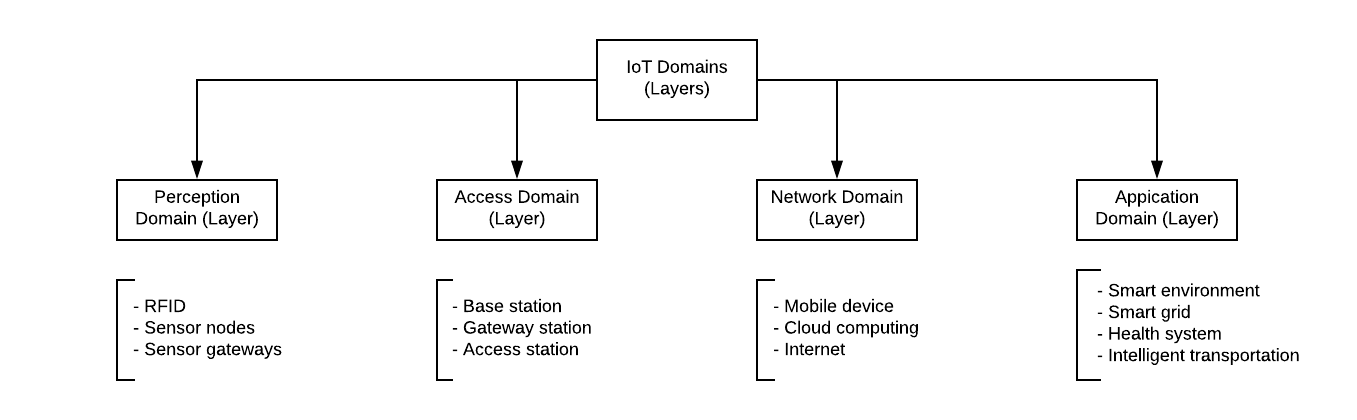
\includegraphics[width=1\textwidth]{IoT_Domains}
		\caption{IoT Domains (Layers).}
		\label{fig:ref_model}
	\end{center}
\end{figure}


\subsubsection{Perception Domain}
Current domain (layer) collects information using readers or gateway. This layer can be divided into two sections:
\begin{enumerate*}[label=(\roman*)]
 \item \textit{perception node}, which is represented by sensors, controllers etc; 
 \item \textit{perception network}, which aim is to interconnect the network domain (layer).  
\end{enumerate*}
Actual reader can extract information from the message received from the RFID tag, which is sticked to the 'thing', while gateway read signals from the sensors, consequently determining the existence of the 'thing' or changes in the environment ~\cite{SSAIoT} ~\cite{IoTSur}.

RFID can be presented as a revolution technology in the embedded communication model, which provides functionality for microprocessors' wireless communication configuration. There are two types of RFID:
\begin{enumerate*}[label=(\roman*)]
 \item \textit{active} - RFID tags with their own power source, which provide signals to readers, creating instant communication; 
 \item \textit{passive} - tiny RFID tags with unique identity to support active communication between tags and readers using wireless networks ~\cite{SSAIoT}.
\end{enumerate*}

Sensor nodes take care of gathering and processing of the sensed data, while being interconnected with other nodes in the network. They have next components:
\begin{enumerate*}[label=(\roman*)]
 \item \textit{controller} - takes care of data processing and other node's parts performance; 
 \item \textit{transceiver} - transmits and receives radio frequencies; 
 \item \textit{program memory} - is used for programming device; 
 \item \textit{power source} - supplies node with power; 
 \item \textit{hardware} - senses data from the environment.
\end{enumerate*}  
 Sensor itself and actuator can be described as the major one components, as they sense data and activate/deactivate device based on commands from the nodes ~\cite{SSAIoT}.

If we look at the wireless networks and how the data is collected from various WSN nodes, we will come to the sensor gateways, which provide above mentioned functionality. Each gateway supports 2.4 GHz IEEE 802.15.4 radio and with a communication framework on board it checks and records the conditions of various sensors. Transmitters and receivers create radio channels between two or more devices to provide data-exchange functionality  ~\cite{SSAIoT}. 

  
\subsubsection{Access Domain}
In the access domain the reader or the head of gateway transfers sensed data to the access point, which is represented by the gateway or base station. Access point then transfers data to the network domain (layer) ~\cite{IoTSur}. 

\subsubsection{Network Domain}
When sensed data leaves access domain (layer), it reaches network domain (layer), which provides network transmission along with information security. "The form of network is possible for any existing network, such as wlan, mobile network, Internet or broadcast and television network" ~\cite{IoTSur}. The network layer consists of mobile devices, clouds and the Internet itself ~\cite{SSAIoT}.

Mobile devices can be characterize as a portable device with its own operating system on board, which supports inbuilt or external applications. These devices are usually equipped with such technologies as Wi-Fi, Bluetooth, Near-Field Communication (NFC), Global Positioning System (GPS) etc. Mobile devices connected to the Internet can provide users with nearly unlimited functionality in digital word. However, they also produce a branch of vulnerabilities, which result into uncounted number of threats to all users' personal data.

Clouds or cloud computing is an Internet-based services, which consist of hardware, systems software, and applications and provides users with resources on-demand. There are three main cloud categories:
\begin{enumerate*}[label=(\roman*)]
 \item \textit{Software as a Service} (SaaS) - user can use an application on-demand, but can not control hardware or network. Such model provide users with applications through the network; 
 \item \textit{Platform as a Service} (PaaS) - allows user to host environment for their applications, however the operating system, hardware or network infrastructure still can not be controlled; 
 \item \textit{Infrastructure as a Service} (IaaS) - gives user an access to ‘fundamental computing resources’ such as CPU, memory, middleware and storage, but cloud infrastructure remains protected ~\cite{Cloud}.
\end{enumerate*}

" The Internet is the global system of interconnected computer networks that use the Internet protocol suite (TCP/IP) to link devices worldwide. It is a network of networks that consists of private, public, academic, business, and government networks of local to global scope, linked by a broad array of electronic, wireless, and optical networking technologies. The Internet carries a vast range of information resources and services, such as the inter-linked hypertext documents and applications of the World Wide Web (WWW), electronic mail, telephony, and file sharing " ~\cite{INT}.


\subsubsection{Application Domain}
 The last domain (layer), but not the least, is the application domain, which can implement the logic in interconnection between ‘things’ and ‘things’ or between ‘things’ and person and plays crucial role in the whole IoT structure as a head layer, which is visible to user and wrap all functionality into User Interface (UI) ~\cite{IoTSur} ~\cite{SSAIoT}. We can allocate four ground types of applications which represent this layer:
\begin{enumerate*}[label=(\roman*)]
  \item \textit{Smart environment} - is represented by intuitively operated devices that help us to organize, structure, and master our everyday life. In other words, smart environments provide functionality, which helps the human to interact with surroundings and reach his goals  ~\cite{SE}; 
  \item \textit{Smart grid} - intelligent power supply network, which provide communication functionality based on two-way wireless and/or wireline communication technologies. Main aim is to increase the productivity and efficiency of the networks. National Institute of Science and Technology (NIST)  considers mobile broadband technologies such as 2G/3G/4G as key enablers for Smart Grid networks, while Electric Power Research Institute (EPRI) examines technologies such as Mobile WiMAX, GPRS and LTE as key enablers for automated metering infrastructure (AMI) ~\cite{SMG}; 
  \item \textit{Healthcare system} - is a framework based on radio frequency technology to deliver sensed data from fragile and accurate micro-nodes embedded inside or outside humans body;
  \item \textit{Intelligent transportation systems (ITS)} - represents a stack of high technology and improvements in information systems, communication, sensors, and advanced mathematical methods interconnected with the surface transportation infrastructure ~\cite{ITS}.
\end{enumerate*}

Each application should be mindful, active and personalized in order to provide secure and stable communication between devices. 
 
\subsection{Taxonomy of the IoT security}

\begin{figure} [H] %try to place the figure here (next option top of the page) 
	\begin{center}
		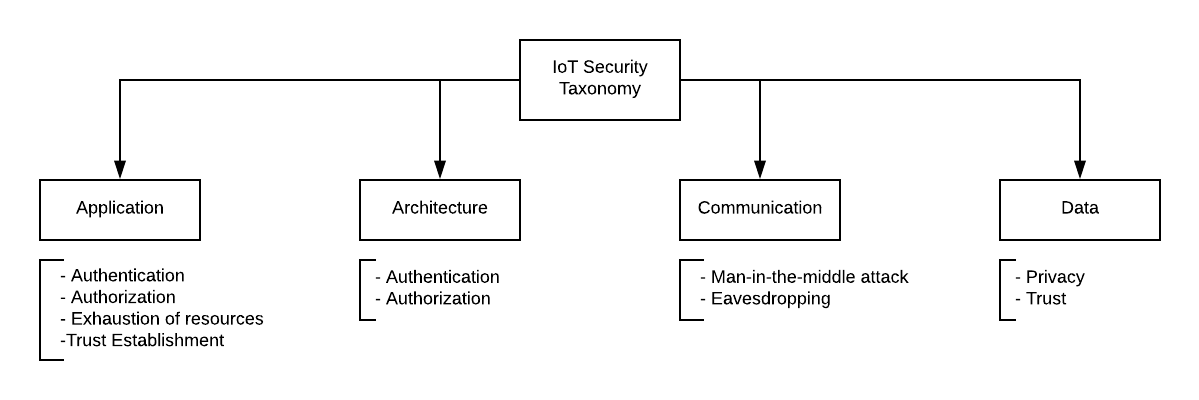
\includegraphics[width=1\textwidth]{IoT_Sec_Tax}
		\caption{IoT Security Taxonomy.}
		\label{fig:ref_model}
	\end{center}
\end{figure}

The existing IoT classification is definitely complicated and heterogeneous, that is why we need to investigate the actual IoT security taxonomy which should be simple and more specifically aimed on characterizing classes of security threats and vulnerabilities in each IoT layer. After studying a branch of existing IoT frameworks ~\cite{SDN/NFV} ~\cite{SEA} ~\cite{SmartC} ~\cite{SOA} ~\cite{Concept} we can allocate four main classes in IoT security, see Figure 2: 
\begin{enumerate*}[label=(\roman*)]
	\item \textit{Application domain} - consists of security techniques such as authentication, authorization, exhaustion  of resources, trust establishment etc;
	\item \textit{Architectural domain} - always depends on the scenarios and application domain. According to ~\cite{IoTSur} ~\cite{SDN/NFV} ~\cite{SEA} ~\cite{SmartC} ~\cite{SOA} ~\cite{Concept} we can provide a summery of existing IoT architectures, see Table 1;
	\item \textit{Communication} - responsible for information exchange/sharing between IoT devices in the system through its layers or between different IoT systems;
	\item \textit{Data} - one of the main targets for threats, its privacy must be guaranteed.
\end{enumerate*}

\newpage
\begin{center}
	\captionof{table}{Examples of existing IoT architectures}
	\tiny
	\begin{longtable}{ p{4cm} p{3cm} p{7cm} }
		\hline\\
		Architecture & Application Domain & Purpose \\[6pt]
		\hline
		\\
		SDN Architecture & Smart environment & SDN manages the network state and the resource allocation, influences the whole system through centralization of the network controller. SDN produces the computing results for an optimized network status  ~\cite{SDN/NFV}. \\[6pt]
		
		NFV Architecture & Smart environment & NFV network functions are implemented with the usage of servers and storage devices of industry standard, which can also be represented by virtual machines. With the reduction of the number of hardware appliances and establishment of the  high volume hardware usage, NFV contributes efficiency and flexibility to the system  ~\cite{SDN/NFV}. \\[6pt]
		
		SEA Architecture & Healthcare & SEA: A Secure and Efficient Authentication and Authorization. SEA accomplishes authentication and authorization of remote end-users using smart e-health gateways. Being relied on the certificate-based DTLS handshake SEA provides secure solution for the medical sensors  ~\cite{SEA}.\\[6pt]
		
		Smart City Architecture & Smart City & The main aim is to combine business architecture, information system architecture and technology architecture into metamodel, which supports consistency, completeness, traceability and relationship of components and layers in the enterprise architecture of the smart city ~\cite{SmartC}.\\[6pt]
			
		Service-Oriented Architecture (SOA) & Smart transportation & SOA defines secure IoT middleware architecture services, which aggregate data streams within the network in order to reduce the overall network load. Although, such architecture enables the interconnection of system elements with different interaction styles. "IoT-based SOA holds the promise of easing the development of rich applications integrating the physical with the virtual worlds in a multitude of domains" ~\cite{SOA}.\\[6pt]
		
		OSCAR: Object Security Architecture & Smart grid & Introduces modern scalable and efficient architecture for E2E security and access control in IoT along with architecture evaluating in M2M settings.\\ [6pt]
		
		Conceptual Organizations Framework & Business organizations & Conceptual Organizations framework " adopts a broad perspective based on User Experience design and attempts to bridge design and system engineering constructs with cognitive and socio-cultural theories, in order to provide a common understanding to multi-disciplinary IoT development teams" ~\cite{Concept}. \\[6pt]
		\hline  
	\end{longtable}
\end{center}

It is clear that in the IoT scenario, security solutions cannot be limited to the single layer, it always has to be an end-to-end combination of overcoming challenges for each class in IoT taxonomy. Consequently, we have to understand the possible issues in each layer in detail as the heterogeneity of IoT interacting objects makes it impossible to construct solution from outside the system, we have to go from inside, combining solutions from different security levels into one strong consequent flow of countermeasures. 

\subsubsection{Security challenges in Application layer}
Major security challenges in the Application layer can be presented by next groups ~\cite{IoTSur}:
\begin{enumerate}[label=(\roman*)]
	\item \textit{Authentication} - allows integration of different IoT devices from different context. During authentication process its required to authenticate routing peers used for data transferring/exchanging along with origin data node authentication. Consequently,  we can affirm that key deployment and key management are ground challenges in IoT authentication ~\cite{IoTCO}. Authentication of nodes is always necessary	for a good and secure implementation as it provides prevention against illegal node access. Authenticating the end to end communication makes the communication secure and the attacker will not be able to spoof the messages between those end hosts. One more challenge is to maintain authentication schemes both lightweight and reliable ~\cite{IoTICA}.   
	\item \textit{Authorization} - addresses the security issue of illegal node access through specifying the access rights to different resources. The data should always be secure protected and accessible only to authorized users. As each IoT node supports limited techniques for access verification it is always challenging to provide appropriate authorization mechanism which will be beneficial and tolerate to nodes with different capabilities ~\cite{IoTSecChel}.   
	\item \textit{Exhaustion of resources} -
	\item \textit{Trust establishment} -
\end{enumerate}

\subsubsection{Security challenges in Architecture}
\subsubsection{Security challenges in Communication}
\subsubsection{Security challenges in Data protection}



\subsection{The future directions in the IoT}



\newpage
\section{Security Risk Management (SRM) } 

\subsection{What is Security Risk Management? }

In general, Security Risk Management  (SRM) can be described as a part of the secure systems development process, which aim is to understand what assets should be protected, from which risks and how these risks could be allayed while covering discovered vulnerabilities of the system  ~\cite{FSSM}. SRM  plays leading role in developing appropriate solutions based on situation and existing security countermeasures. Typically it provides a set of rules to lower the risk level or totally prevent possible attacks on the system along with the hints for successfully and qualitative system monitoring. There are many different methodologies which apply SRM in various domains, that's why deep understanding of the system's architecture is crucial during SRM analytical procedure.

According to ~\cite{FSSM} we will look at a few of SRM methods as the number of existing approaches always grow and we can not pretend our survey to be complete. However, chosen SRM methods should  be enough to understand what king of analysis concepts and principles are used during analytical procedure in security risk management.

\textit{CORAS} is a risk assessment methodology ~\cite{CORAS} which provides detailed instructions for the use of UML-oriented modelling for the next three main purposes:
\begin{enumerate*}[label=(\roman*)]
  \item "to describe the target of assessment at the right level of abstraction"~\cite{CORAS}.
  \item "as a medium for communication and interaction between different groups of stakeholders involved in risk assessment"~\cite{CORAS}.
  \item "to document risk assessment results and the assumptions on which these results depend"~\cite{CORAS}.
\end{enumerate*}
There are three ground steps for the risk analysis of the \textit{CORAS} risk management process:
\begin{enumerate*}[label=(\roman*)]
	\item identify risks;
	\item analyse risks;
	\item evaluate risks.
\end{enumerate*} 
The \textit{CORAS} risk management process based on using branch of approaches in terms of XML technology for analysing different parts of the system independently. The choice of the method is made by evaluating the viewpoint in which the part to be analysed appears and  determining development lifecycle phase. 

\textit{EBIOS}  (French: Expression des Besoinset Identification des Objectifs de Securite) is a method for analysing, evaluating and counter-measuring against risks in the system. There are five main steps of the \textit{EBIOS} method ~\cite{EBIOS}:
\begin{enumerate*}[label=(\roman*)]
	\item Circumstantial study - determining the context;
	\item Security requirements;
	\item Risk valuation;
	\item Security goals determination; 
	\item Identification of security requirements.
\end{enumerate*}
According to ~\cite{EBIOS} \textit{EBIOS}  generates a security policy adapted to the system based on its specifications and features. The method was created in 1995 and is now maintained by the ANSSI, a department of the French Prime Minister.

\textit{AURUM} (Automated Risk and Utility Management) is a framework for information security risk management ~\cite{AURUM}, which was developed to help in decision making according to organisational needs with respect to selection of security measures. It represents a new methodology for supporting the NIST SP 800-30 risk management standard. According to ~\cite{AURUM} the next benefits were documented: 
\begin{enumerate*}[label=(\roman*)]
	\item \textit{AURUM} provides risk manager with an "ontological information security knowledge base" in order to structure the information security knowledge in appropriate way;
	\item Describes the methodology for the consistent modelling of organizational resources;
	\item Provides guidelines for using "widely accepted
information security knowledge for threat/vulnerability
identification and control recommendations"~\cite{AURUM};
	\item Introduces usage of the Bayesian threat likelihood determination, which gives opportunity for the objective level threat evaluation;
	\item Automated threat impacts calculation as a part of system's resources rating;
	\item Automated controls proposals for the risks mitigation; 
	\item Provides risk manager with an opportunity to investigate possible scenarios and characterize  the problem in details; 
\end{enumerate*} 

\textit{MEHARI} (MEthod for Harmonized Analysis of RIsk) is a free risk management method for the information systems. This framework combines complex knowledge base with existing tools into the powerful instrument for the information security risk analysis ~\cite{MEHARI}. There are next ground steps:
\begin{enumerate*}[label=(\roman*)]
	\item Threat analysis;
	\item Business process analysis;
	\item System assets classification;
	\item Risks ratio processing;
	\item Diagnostic questionnaires for evaluation risks' mitigation level of the system;
	\item System Security Requirements evaluation;
	\item Possible scenarios determination;
	\item Developing countermeasures based on possible risks scenarios;
\end{enumerate*}
Entire focusing on the risks analysing and creating controls makes \textit{MEHARI} a powerful framework for the SRM.

\textit{CRAMM} (CCTA Risk Analysis and Management Method) is an automated tool based on qualitative risk assessment methodology, which consists of the next stages ~\cite{CRAMM}:
\begin{enumerate*}[label=(\roman*)]
	\item Assets identification and evaluation;
	\item Threat and vulnerability assessment;
	\item Countermeasures recommendation;
\end{enumerate*}
As it mentioned in ~\cite{CRAMM}  "CRAMM is a comprehensive and flexible tool especially for justifying prioritized countermeasures at a managerial level, needing, however, qualified and experienced practitioners for efficient results".



\subsection{Domain Model for SRM}

One of the most important role in Security Risk Management (SRM) is played by the SRM Domain Model. The main purpose of a domain model is to represent the main concepts of the system with their responsibilities and relationships. Based on main features of the concepts, we can then classify  them as different assets ~\cite{IoTRefMod}. In this way we can determine what assets need to be protected and from which risks. Such strategy  helps to generalize understanding of the system's problem between people who are working on possible solutions for it. Only with a common understanding of the main concepts it becomes possible to argue about architectural solutions and to evaluate them.
 
We have  SRM domain model (SRMDM) represented as an UMl diagram on the Figure 1. All elements of the SRMDM could be divided into three major groups ~\cite{FSSM}: 
\begin{enumerate*}[label=(\roman*)]
	\item \textit{asset-related concepts} - "describe which of an organisation’s assets are important to protect and what criteria guarantee a certain level of asset security" ~\cite{FSSM}. Typically pure \textit{asset} can be represented by any part of the system which has some value and plays a role in the work of whole system. Assets can also be divided into sub-groups: \textit{business assets} ("describes the information, processes, capabilities and skills essential to the business and its core mission"  ~\cite{FSSM})  and \textit{organizational assets}, which are represented by the core elements of the system and play crucial role in providing appropriate service to the customers;
	\item \textit{risk-related concepts} - "introduce definitions of risk itself and its immediate components" ~\cite{FSSM}. According to the Figure 1 we can allocate \textit{risk} itself as a combination of the \textit{threat} which exploits existing \textit{vulnerability} of the system plus \textit{impact} to which such \textit{event} can lead to.;
	\item \textit{risk treatment-related concepts} - "describe the concepts to treat risk"  ~\cite{FSSM}. According to  ~\cite{FSSM} we can choose one of four ground risk treatment decisions while risk mitigating process: \textit{Risk avoidance} - describes approach of modifying system's functionality to fully avoid possible risk; \textit{Risk reduction} - proposes strategy of the minimization risk occurrence possibility, so security requirements are, typically, selected for
	reducing the risks instead of full avoidance; \textit{Risk transfer} - "defines how risk parties could share the burden of loss from a risk"  ~\cite{FSSM}; \textit{Risk retention} - "constitutes acceptance of the burden of loss from a risk. No design decision is necessary in this case." ~\cite{FSSM}. 
\end{enumerate*} 


 
\begin{figure} [H] %try to place the figure here (next option top of the page) 
	\begin{center}
		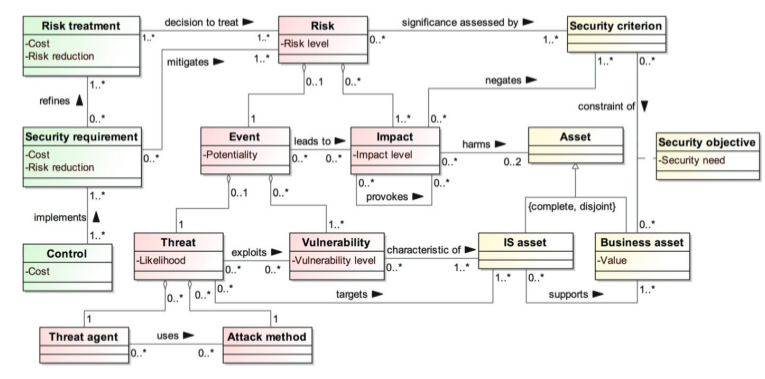
\includegraphics[width=1\textwidth]{SRM_Domain}
		\caption{General SRM Domain Model.}
		\label{fig:ref_model}
	\end{center}
\end{figure}

\newpage
\section{Content and Assets of IoT}
The Internet of things (IoT) is represented by wisely connected devices and systems to exchange or accumulate and process data generated by users or by embedded sensors and actuators in machines and other physical objects. IoT starts playing leading role in improving customers' life quality on different layers including security, health, education and energy efficiency. Industrial business has also experienced advantages of using IoT systems in manufacturing, retail, agriculture and other sectors ~\cite{UnderIoT}.

As the IoT through last years has gained a significant positive impact on consumers, enterprises and society as a whole it also has bring in a stack of risks connected to  beneficial services provided by IoT systems. That's why we need to understand a General Domain Model Architecture of the IoT (GDMA)  ~\cite{GDMA} in order to establish the common grounding definition of IoT system assets and to describe their basic interactions  and relationships with each other.

\subsection{IoT Domain Model}

 
 Internet of Things Domain Model (IoTDM) plays leading role in applying SRM methods to the IoT systems since it provides definition of the main abstract concepts of the system. The Domain Model helps to determine system and business assets of the IoT system and then evaluate their importance in order to apply appropriate countermeasures against existing risks. "The main purpose of a domain model is to generate a common understanding of the target domain in question" ~\cite{IoTRefMod}. 
 
 
 \begin{figure} [H] %try to place the figure here (next option top of the page) 
	\begin{center}
	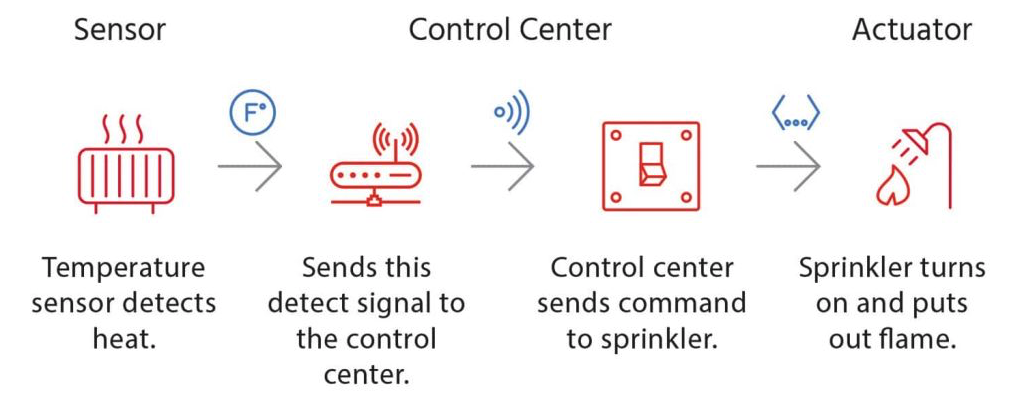
\includegraphics[width=1\textwidth]{simple}
	\caption{Sensor to Actuator work flow.}
	\label{fig:ref_model}
	\end{center}
	\end{figure}
	
\newpage
 Figure 3 shows us general IoTDM which we will use while applying SRM to the existing IoT system. However, before describing how we will secure real system and from which risks we have to describe our IoTDM in terms of SRM and determine relationships between concepts represented in both domain models. 
 
     
 \begin{figure} [H] %try to place the figure here (next option top of the page) 
	\begin{center}
	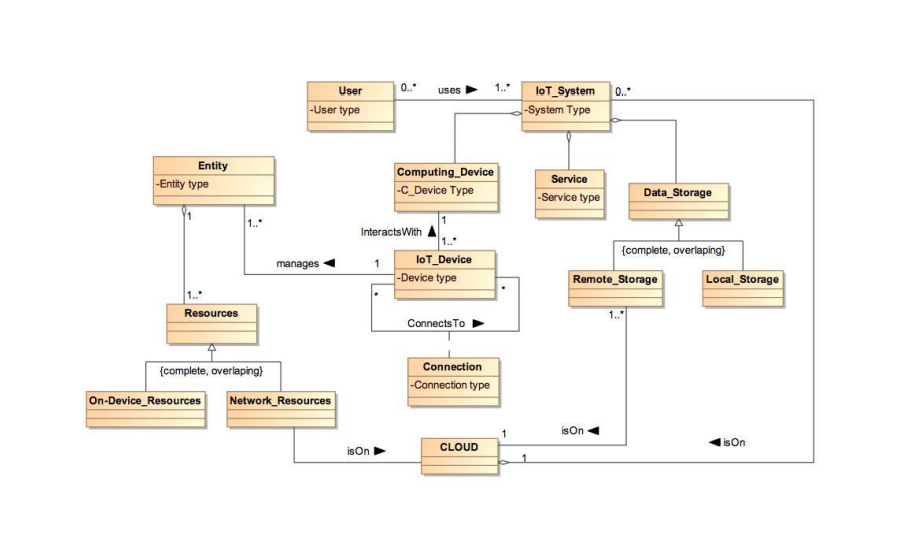
\includegraphics[width=1\textwidth]{IoT_Domain_Model}
	\caption{General Domain Model Architecture of the IoT.}
	\label{fig:ref_model}
	\end{center}
	\end{figure}
	
 Lets represent the initial work flow of the simple IoT system in terms of SRM. If we look at Figure 2 we can determine four IoT elements:
 \begin{enumerate*}[label=(\roman*)]
 	\item \textit{temperature sensor} - detects heat;
	\item \textit{Wi-Fi module} - sends detected temperature from the sensor to the \textit{control center};
	\item \textit{control center} - makes decision what command should be sent to the sprinkler based on the previously received temperature from the \textit{temperature sensor}; 
	\item \textit{actuator} - represented by sprinkler, turns on and puts out flame or turns off depending on the command from the \textit{control center}. 
 \end{enumerate*}
Suppose, an attacker, (\textit{Threat agent}) with means to break a normal work flow of our IoT system from Figure 3, exploits the weakness of the Wi-Fi connection between Wi-Fi module and Control center, which represent \textit{System assets}, and get an access to the temperature (\textit{Business asset}) which is going from the sensor. Then an attacker changes the temperature value and this \textit{Event} leads to the \textit{Impact} of overheating and consequently to the \textit{Harm} to sprinkler. Such \textit{Event} and its \textit{Impact} represent \textit{Risk} to the IoT system. 

Finally, we can summarize that assets in the IoT represent anything that is valuable for the IoT system or play crucial role in providing appropriate functionality and services to users. According to  ~\cite{FSSM} \textit{system assets} can be described as parts of the IoT system, which gain their importance through supporting business assets. Typically, system assets in IoT can be represented as ground components of the information technology system such as hardware, software or network. In our simple example from Figure 2 system assets are represented by sensor, Wi-Fi module, Control center and Actuator. 

\textit{Business assets} are extremely valuable for each IoT system as they represent essential to the business things such as information,  processes, capabilities and skills ~\cite{FSSM}. Besides official definitions, business assets can be commonly represented by the data, which is transferred, stored or manipulated by the IoT system during working process. As a result business assets security is definitely worth attention. According to Figure 3 business assets are represented by the temperature which goes from  the Sensor to the Control center and commands from the Control center to the Actuator.  
\vspace*{1ex}


\newpage
\subsection{Vulnerability}
According to the cyber-security terms we can determine vulnerability as a " term that refers to a flaw in a system that can leave it open to attack. A vulnerability may also refer to any type of weakness in a computer system itself, in a set of procedures, or in anything that leaves information security exposed to a threat "  ~\cite{V} . In terms of Security Risk Management applied to the IoT  vulnerability is a characteristic of the system asset or group of IS assets that exposes a weakness or flaw in terms of security ~\cite{FSSM}. 

Have to be mentioned that if we talk about vulnerability of the application, then it could be presented as a weakness in design flaw or an implementation bug, which can allow an attacker to harm application owner, application users, and other entities that rely on the application. According to the Open Web Application Security Project ~\cite{OWASP} we can allocate next most common IoT vulnerabilities:
\begin{enumerate}
	\item \textbf{Insecure Web Interface, V\#1:}
		\newline \textit{Threat agent} - an attacker with access to the web interface. Could be presented by external or internal user of the system.
		\newline \textit{Attack method} - an attacker uses weak credentials, gains access to plain-text credentials or enumerates accounts to access the web interface.
		\newline \textit{Vulnerability} - account enumeration, lack of account lockout or weak credentials	are the most common vulnerabilities of the insecure Web Interface.
		\newline \textit{How to discover} - issues of the Web Interface could be find out during manual work with the system along with using testing tools for cross-site scripting identification.
		\newline \textit{Impact to system assets} - insecure web interface could result in harm to service’s data confidentiality, integrity and availability which can then lead to complete device takeover.
		\newline \textit{Impact to business assets} - the actual device or whole IoT System could be compromised along with the users.
		\newline \textit{Possible attack examples}:
			\begin{enumerate}[label=(\roman*)]
				\item The Forgot Password functionality provides responses on entering invalid users’ credentials. As soon as valid credentials identified an attacker could calculate appropriate password using
				brood force methods.
				\item Web interface maintains vulnerable to cross site scripting. For example, the HTML snippet: 
			\end{enumerate}
	\item  \textbf{Insufficient Authentication/Authorization, V\#2:}
		\newline \textit{Threat agent} - an attacker with access to the web interface. Could be presented by external or internal user of the system.
		\newline \textit{Attack method} - an attacker uses weak passwords, insecure password recovery mechanisms, poorly protected credentials or lack of granular access control to access a particular interface.
		\newline \textit{Vulnerability} - weak passwords or credentials with poor protection can lead to insufficient authentication.
		\newline \textit{How to discover} - common issues with authentication/authorization can be discovered while examining the interface of the system with automated testing and require more stable passwords.
		\newline \textit{Impact to system assets} - insufficient authentication/authorization can result into harm to system’s data confidentiality, integrity and availability or denial of access.
		\newline \textit{Impact to business assets} - all users could be compromised as a result of their data being stolen.
		\newline \textit{Possible attack examples}:
			\begin{enumerate}[label=(\roman*)]
				\item The interface requires simple passwords.
				\item Users’ credentials are not appropriate protected while transmission to the DB or not encrypted before sending.
			\end{enumerate}
	\item \textbf{Insecure Network Services, V\#3:}
		\newline \textit{Threat agent} - an attacker with a network access to the IoT device. Could be internal or external user.
		\newline \textit{Attack method} - an attacker uses vulnerabilities in network services to launch an attack on IoT device itself or bounce attacks off the device.
		\newline \textit{Vulnerability} - not enough controls on open ports and traffic monitoring in the system.
		\newline \textit{How to discover} - insecure network services can often be detected with the help of port scanners tools and fuzzers. " Fuzzing or fuzz testing is an automated software testing technique that involves providing invalid, unexpected, or random data as inputs to a computer program. The program is then monitored for exceptions such as crashes, or failing built-in code assertions or for finding potential memory leaks. Typically, fuzzers are used to test programs that take structured inputs." [\url{https://en.wikipedia.org/wiki/Fuzzing}].
		\newline \textit{Impact to system assets} - insecure network can result into harm to system’s data confidentiality, integrity and availability or denial of service. Can also be a reason for launching attacks on other systems’ devices.
		\newline \textit{Impact to business assets} - denial of service attack could lead to users’ data loss of availability along with data loss.
		\newline \textit{Possible attack examples}:
			\begin{enumerate}[label=(\roman*)]
				\item Fuzzing attacks. Lets consider an example of fuzzing attack with a Burp Suite Intruder and an OWASP WebGoat application. An attacker here with means to log into the app as Admin user
				without the password.
				\item Some ports are open and are not monitored by the system, so could be accessed via UPnP.
			\end{enumerate}
	\item \textbf{Lack of Transport Encryption, V\#4:}
		\newline \textit{Threat agent} - an attacker with an access to the network the IoT device is connected to.
		\newline \textit{Attack method} - attacker uses the lack of transport encryption to view data being passed over the network.
		\newline \textit{Vulnerability} - lack of transport encryption is a common vulnerability for local networks as it is assumed that in the local and wireless networks the traffic will not be widely visible and accessible. However it makes all the data transferred through such networks visible for possible attacker in range of the wireless network support or with external access to the local network.
		\newline \textit{How to discover} - many issues with transport encryption are easy to discover simply by launching testing attack on the system with viewing network traffic and searching for readable data in it. An automated tools can also look for proper implementation of common transport encryption such as SSL and TLS.
		\newline \textit{Impact to system assets} - insecure web interface could result in harm to service’s data confidentiality, integrity and availability which can then lead to complete device takeover.
		\newline \textit{Impact to business assets} - the actual device or whole IoT System could be compromised along with the users.
		\newline \textit{Possible attack examples}:
			\begin{enumerate}[label=(\roman*)]
				\item The cloud interface uses only HTTP.
				\item User-name and password are transmitted in the clear over the network.
			\end{enumerate}
	\item \textbf{Privacy Concerns (Confidentiality), V\#5:}
		\newline \textit{Threat agent} - an attacker with an access to the IoT device itself, the network the device is connected to, the mobile application and the cloud connection.
		\newline \textit{Attack method} - an attacker uses insufficient authentication, lack of transport encryption or insecure network services to break systems’ data confidentiality.
		\newline \textit{Vulnerability} - all vulnerabilities of authentication/authorization, low protected transport protocols and not appropriate secure network services.
		\newline \textit{How to discover} - privacy concerns are easy to discover by simply reviewing the data that is being collected as the user sets up and activates the device. Automated tools can also look for specific patterns of data that may indicate collection of personal data or other sensitive data.
		\newline \textit{Impact to system assets} - harm to service’s data confidentiality, integrity and availability which can then lead to complete device takeover.
		\newline \textit{Impact to business assets} - the actual device or whole IoT System could be compromised along with the users.
		\newline \textit{Possible attack examples}:
		\begin{enumerate}[label=(\roman*)]
			\item Collection of personal data.
			\item Collection of financial and/or health information.
		\end{enumerate}
	\item \textbf{Insecure Cloud Interface, V\#6:}
		\newline \textit{Threat agent} - an attacker with an access to the internet.
		\newline \textit{Attack method} - an attacker uses insufficient authentication, lack of transport encryption and account enumeration to access data or controls via the cloud interface (website).
		\newline \textit{Vulnerability} - low level security of the cloud access credentials or account enumeration is possible.
		\newline \textit{How to discover} - insecure cloud interfaces are easy to discover by simply reviewing the connection to the cloud interface and identifying if SSL is in use or by using the password reset mechanism to identify valid accounts which can lead to account enumeration.
		\newline \textit{Impact to system assets} - harm to service’s data confidentiality, integrity and availability	which can then lead to complete device takeover.
		\newline \textit{Impact to business assets} - the actual device or whole IoT System could be compromised along with the users.
		\newline \textit{Possible attack examples}:
		\begin{enumerate}[label=(\roman*)]
			\item Password reset indicates whether account is valid.
			\item User-name and password are poorly protected when transmitted over the network. In such cases, an attacker is able to either determine a valid user account or capture the credentials as they cross the network and decode them since the credentials are only protected using	Base64 Encoding.
		\end{enumerate}
	\item \textbf{Insecure Mobile Interface, V\#7:}
		\newline \textit{Threat agent} - an attacker with access to the mobile application.
		\newline \textit{Attack method} - an attacker uses insufficient authentication, lack of transport encryption and account enumeration to access data or controls via the mobile interface (application).
		\newline \textit{Vulnerability} - low level security of the app access credentials or account enumeration is possible.
		\newline \textit{How to discover} - insecure mobile interfaces are easy to discover by simply reviewing connection to the wireless networks and identifying if SSL is in use or by using the password reset mechanism to identify valid accounts which can lead to account enumeration.
		\newline \textit{Impact to system assets} - harm to service’s data confidentiality, integrity and availability which can then lead to complete device takeover.
		\newline \textit{Impact to business assets} - the actual device or whole IoT System could be compromised along with the users.
		\newline \textit{Possible attack examples}:
		\begin{enumerate}[label=(\roman*)]
			\item Password reset indicates whether account exist or not.
			\item User-name and password are poorly protected when transmitted over the network. In such cases, an attacker is able to either determine a valid user account or capture the credentials as they cross the network and decode them since the credentials are only protected using Base64 Encoding.
		\end{enumerate}
	\item \textbf{Insufficient Security Configurability, V\#8:}
		\newline \textit{Threat agent} - an attacker with an access to the IoT device.
		\newline \textit{Attack method} - an attacker uses the lack of granular permissions to access data or controls on the device, low level transport encryption and the use of low level passwords can also be the doors for the attack on the system.
		\newline \textit{Vulnerability} - insufficient security configurability is present when users of the device have limited or no ability to alter its security controls. If the web interface does not support creating granular user permissions and does not force user for creating strong password.
		\newline \textit{How to discover} - detailed review of the web interface along with provided options can reveal existing vulnerability.
		\newline \textit{Impact to system assets} - harm to service’s data confidentiality, integrity and availability	which can then lead to complete device takeover.
		\newline \textit{Impact to business assets} - the actual device or whole IoT System could be compromised along with the users. 
		\newline \textit{Possible attack examples}:
		\begin{enumerate}[label=(\roman*)]
			\item Strong passwords are not forced to be used, then an attacker is able to gain access to existing accounts using brood force methods.
			\item Valuable data which is stored on the device is not encrypted, then an attacker is able to access data at rest which has just simple protection such as asking for administrator’s credentials to view data.
		\end{enumerate}
	\item \textbf{Insecure Software/Firmware, V\#9:}
		\newline \textit{Threat agent} - an attacker with an access to the IoT device and/or network the device connects to and/or the server which provides updates to the IoT devices Software.
		\newline \textit{Attack method} - an attacker captures files with updates from unencrypted connection between server and ioT devices. The files with updates are not encrypted itself. An attacker performs unauthorized update of the system software via DNS hijacking.
		\newline \textit{Vulnerability} - low system states monitoring, low level encryption. Devices should have the ability to be updated when vulnerabilities are discovered and software/firmware updates can be insecure when the updated files themselves and the network connection they are delivered on are not protected. Software/Firmware can also be
		insecure if they contain hardcoded sensitive data such as credentials.
		\newline \textit{How to discover} - security issues with software/firmware are relatively easy to discover by simply inspecting the network traffic during the update to check for encryption or using a hex editor to inspect the update file itself for interesting information.
		\newline \textit{Impact to system assets} - harm to service’s data confidentiality, integrity and availability which can then lead to complete device takeover.
		\newline \textit{Impact to business assets} - the actual device or whole IoT System could be compromised along with the users.
		\newline \textit{Possible attack examples}:
		\begin{enumerate}[label=(\roman*)]
			\item Update file is transmitted via HTTP then an attacker is able to change them on their way from server to device.
			\item Update file is unencrypted and human readable data can be viewed.
			
			In the cases above, the attacker is able to either capture the update file or capture the file and view it's contents.
		\end{enumerate}
	\item \textbf{Poor Physical Security, V\#10:}
		\newline \textit{Threat agent} - an attacker who has physical access to any physical system asset.
		\newline \textit{Attack method} - an attacker uses vectors such as USB ports, SD cards or other storage means to access the Operating System and potentially any data stored on the device.
		\newline \textit{Vulnerability} - Physical security weaknesses are present when an attacker can disassemble a device to easily access the storage medium and any data stored on that medium. Weaknesses are also present when USB ports or other external ports can be used to access the device using features intended for configuration or maintenance.
		\newline \textit{How to discover} - detailed review of the hardware components of the IoT system.
		\newline \textit{Impact to system assets} - harm to service’s data confidentiality, integrity and availability	which can then lead to complete device takeover
		\newline \textit{Impact to business assets} - the actual device or whole IoT System could be compromised along with the users.
		\newline \textit{Possible attack examples}:
		\begin{enumerate}[label=(\roman*)]
			\item The device can be easily disassembled and storage medium is an unencrypted SD card.
			\item USB ports are present on the device then an attacker is able to change device software or stole valuable data from it.
		\end{enumerate}
\end{enumerate}    
\vspace*{1ex}


\subsection{IoT Security Controls } 
During SRM process in IoT determining possible risks is not the only step in securing system. It is always important to know how to cover existing vulnerabilities in order to mitigate possible risks. In the IoT, securing process requires a holistic understanding of security controls for all assets of the system. Security mechanism should be unique for each valuable element of the system as it has to follow elements' lifecycle and functionality provided to the system. In this section we allocate and describe ground keys in securing IoT systems and propose appropriate contermasures for covering different types of systems' vulnerabilities ~\cite{SecIoT}.

\subsubsection{Protocol and network security} 
Protocol and network security often requires optimizations in cryptography algorithms and appropriate key management systems, as cryptography plays leading role in developing security protocols for securing network infrastructure. However, applying standard Internet security mechanisms  to the functional assets of the  IoT system could be inefficient due to the lack of the assets' resources. Therefore, security protocols should be adapted based on the assets' architecture taking into account their performance and capabilities. 
According to the Open Web Application Security Project ~\cite{OWASP} we can propose next security countermeasure to apply protocol and network security on appropriate level: 
\begin{enumerate}
\item \textbf{Secure Network Services, Cm\#1:}
		\begin{itemize}
			\item Only necessary ports which are crucial for the appropriate system functionality should be exposed and available.
			\item Service should be protected from buffer overflow (overrun) ~\cite{BufOver} and fuzzing attacks ~\cite{FuzA}.
			\item Ensure that the service is prepared and not vulnerable to DoS attacks ~\cite{DoS} or at least monitoring system is provided to determine such type of an attack.  
			\item Ensure that network ports and services exposed to the internet via UPnP for example.
			\item Monitoring system should also detect abnormal service request traffic and block gateways if necessary. 
		\end{itemize}
		
 \item \textbf{Transport Encryption, Cm\#2:}
		\begin{itemize}
			\item Always use transport protocols such as SSL ~\cite{SSL/TLS} and TLS ~\cite{SSL/TLS} while data transferring through network to be sure that your data is encrypted. 
			\item If SSL or TLS are not available do not hesitate to use other standard encryption methods to protect data. 
			\item Pay attention what encryption techniques are used. Avoid using unaccepted encryption standards.
			\item Use MQTT payload encryption ~\cite{MQTT} to protect system's specific data on the application level.
			\item Ensure to use secure encryption key handshaking.
			\item Always verify incoming data for integrity. 
		\end{itemize}
\end{enumerate}

Countermeasure on secure network services (Cm\#1) mitigate risks with vulnerabilities of insecure network services (V\#3), and communication encryption
(Cm\#2) – vulnerabilities related the lack of communication encryption (V\#4).

\subsubsection{Data and privacy} 
Data and privacy key often represented by the most sensitive and valuable assets of the IoT system. Each user wants their personal data be protected and managed by themselves, but there are a lot of  systems which based on managing users' data. In such cases a huge issue is to constrain and monitor the list of accepted data managers. Consequently, using cryptographic algorithms and different protocols for secure data transferring could be not enough.  In other words it should be developed special management policy based on the data type managed by the system. We can propose next countermeasures ~\cite{OWASP}:
\begin{enumerate}
	\item \textbf{Privacy Concerns, Cm\#3:}
		\begin{itemize}
			\item While collecting data be sure that:
				\begin{enumerate*}[label=(\roman*)]
					\item only critical to the functionality of the system data is collected;
					\item avoid collecting sensitive data;
					\item collected data is de-identified or anonymized;
					\item retention limits are set for the collected data;
					\item protect collected data with encryption.
				\end{enumerate*}
			\item Ensure that personal information is properly protected on all levels of the system.
			\item Give access to the collected data only for authorized users.
			\item Do not collected more data that actually needed for appropriate functionality of the system.
			\item Always de-identify data before analyzing.
		\end{itemize}
	\item \textbf{Secure Software/Firmware, Cm\#4:}
		\begin{itemize}
			\item Ensure that the system uses secure update mechanism and all files transferring is based on accepted encryption methods.
			\item The update file should not expose sensitive data.
			\item Each pack of incoming files with updates should be signed and verified before even saving in system memory storage.
			\item Use only trusted and secure servers for updates.
			\item If possible, its recommended to use secure boot ("Secure Boot is a technology where the system firmware checks that the system boot loader is signed with a cryptographic key authorized by a database contained in the firmware." ~\cite{SB}).
		\end{itemize}
	\item \textbf{Physical Security, Cm\#5:}
		\begin{itemize}
			\item Use only trusted and protected data storage services that can not be easily removed.
			\item All sensitive system's data should be encrypted at rest.
			\item  Always check that USB ports or other external ports are protected from uploading malicious software through.
			\item It is recommended to minimize the number of external ports such as USB used by the system.
			\item "Ensuring the product has the ability to limit administrative capabilities" ~\cite{OWASP}.
		\end{itemize}
\end{enumerate}

Countermeasures regarding the privacy concerns (Cm\#3) help to mitigate
security risks with vulnerabilities related to privacy concerns (V\#5); secure
software and/or firmware (Cm\#4) – vulnerabilities related to insecure software
and/or firmware (V\#9). Countermeasure of physical security (Cm\#5) address
risks with vulnerabilities of poor physical security (V\#10).

\subsubsection{Identity management} 
Identity management represents a non-trivial process of verifying a staggering variety of identity and connection types. We can allocate a key rules which should be followed during IoT system identity management:
  		\begin{enumerate}
 			 \item An object's identity should always be unique compared to the other objects from its family.
			 \item Unique identity can be called core identity, as an object can also have several temporary identities. 
			 \item  Self-identification is one of the ground features of an object.
			 \item An object knows the identity of its owner if it exists.
		\end{enumerate}
One more important mechanism in identity management is to give an object opportunity to cover its identity if needed.  As IoT systems cover different backgrounds of the humans' everyday life, there are situations when it is not safe to reveal identities only based on incoming requests. If look more precise at Identity management we can propose to follow next recommendations:
\begin{enumerate}
	\item \textbf{Secure Authentication/Authorization, Cm\#6:}
		\begin{itemize}
			\item Ensure that strong usernames and passwords are always required.
			\item Two factor authentication and users' credentials encryption should be implemented if possible.  
			\item Be aware of insecure  password recovery mechanisms and be sure that "re-authentication is required for sensitive features" ~\cite{OWASP}.
			\item Revoking mechanism should be developed for the system's credentials.
			\item Application, device and server authentication are always required.
			\item "Manage authenicated user id(credential info.) and the user's device id, the user's app id mapping table in the authentication server" ~\cite{OWASP}.
			\item Authentication token/session should always be unique to each user along with  user id, app id and device id.
		\end{itemize}
			\item \textbf{Secure Web Interface, Cm\#7:}
		\begin{itemize}
			\item Default username and password should be non trivial and its recommended to change them during initial setup.
			\item "Forgot password" functionality should be secure and sturdy. Be sure that you do not provide user with information indicating valid account.
			\item Always check if your Web Interface is protected from XSS (Cross-site Scripting) ~\cite{XSS}, SQLi (SQL injections) ~\cite{SQLi} or CSRF (Cross-site request forgery) ~\cite{CSRF};
			\item Do not hesitate to use only encrypted transport protocols while transferring system's credentials.
			\item Do not allow usage of low level passwords.
			\item Set appropriate number of attempts that allowed while logging in to the system. If the number was exceeded it is recommended temporary block the user for further authentication procedures if needed. 
		\end{itemize}
			\item \textbf{Secure Mobile Interface, Cm\#8:}
		\begin{itemize}
			\item Default usernames and passwords should always be changed during initial setup.
			\item Ensure you system is protected from account enumeration through password reset mechanisms
			\item Set a limit for unsuccessful login attempts, so if it was reached the user is temporary blocked.
			\item Try not to transfer system's credentials over the internet.
			\item Two factor factor authentication should be implemented.
			\item Its recommended to use obfuscation technique ~\cite{CO} applied to mobile app of the system.
			\item Restrict the mobile app's execution on tempered OS environment" ~\cite{OWASP}.
		\end{itemize}
\end{enumerate}

Countermeasures to secure authentication and/or authorization (Cm\#6) mitigate risks with vulnerabilities of insufficient authentication and/or validation (V\#2); to secure Web interface (Cm\#7) – vulnerabilities of insecure Web interface (V\#1); and to secure mobile interface (Cm\#8) – vulnerabilities of insecure mobile interface (V\#7).

\subsubsection{Trust and governance, Cm\#9:} 
Trust and governance the fundamentals in each IoT system. Represented by mechanism which dynamically  evaluates objects  it helps to control users' services based on the interaction process. In pair with governance trust play role of a framework which key role is to support cohesion and stable work of the security protocols in the system. This key plays crucial role for the systems which services rely on Cloud interface. According to ~\cite{OWASP} we can recommend next countermeasures:
\begin{itemize}
			\item Default usernames and passwords should always be changed during initial setup.
			\item Ensure you system is protected from account enumeration through password reset mechanisms.
			\item Set a limit for unsuccessful login attempts, so if it was reached the user is temporary blocked.
			\item Cloud-based interface should be always protected from XSS (Cross-site Scripting) ~\cite{XSS}, SQLi (SQL injections) ~\cite{SQLi} or CSRF (Cross-site request forgery) ~\cite{CSRF};
			\item Try not to transfer system's credentials over the internet.
			\item Two factor factor authentication should be implemented.
			\item Monitoring system should detect abnormal service request traffic and block gateways if necessary.
		\end{itemize}

Countermeasures regarding the trust and governance (Cm\#9) deal with the security risks with vulnerabilities of insecure cloud interface (V\#6).
 
\subsubsection{Fault tolerance, Cm\#10:} 
 Clearly, no IoT system can pretend to be entirely secure, since the number of possible threads rising significantly faster then the number of solutions for covering new-appeared vulnerabilities in the system. Accomplishing acceptable fault tolerance in IoT requires next interdependent efforts:
 		\begin{enumerate}
 			\item All objects have to be secure by default, it means that beside secure protocols and algorithms the comprehensive software structure should always be improved.
 			\item The state of the network and its services should be shared among all IoT objects. This will provide an opportunity to maintain states' monitoring management on appropriate level as each object would be able to associate its own state changes with the network state changes. Constituently, the system monitoring quality will grow up.
 			\item Based on the second effort, each object should be able to protect themselves if the network state said about network collapse or attack. To arrange this functionality intrusion-detection system should be introduced as well as other defensive structures.
 			\item Force system to separate  normal users from administrative users.
			\item Provide functionality to encrypt data data at rest or in transit.
			\item Force users to use only strong passwords during authorization/authentication processes.
			\item "Ensuring the ability to enable logging of security events and to notify end users of security events" 
 		\end{enumerate}
 

Countermeasures regarding the fault tolerance (Cm\#10) mitigate security risks with vulnerabilities of insufficient security configurability (V\#8).

\newpage
\section{Analysis of Security Risks in IoT Systems}

In this section we discuss few reported examples. The purpose is to illustrate the IoT assets, risks, and their vulnerabilities; potentially the countermeasures discussed in Section 3 should be applied to mitigate these risks.


\begin{adjustbox}{angle=90}
	\begin{tabular}{ | l | p{5cm} | p{5cm} | p{5cm} |}
		\hline
		& Example 1 ~\cite{Ex1} & Example 2 ~\cite{Ex2} & Example 3 ~\cite{Ex3} \\ \hline
		Threat agent &  An attacker with means to break normal work flow of the popular web services.
		& 
		An attacker with means to interrupt heating process of the buildings. 
		& 
		An attacker with means to slow down the work flow of the university servers.  \\  \hline
		Attack method & 1)  Infection IoT devices using Mirai botnet;
		2) Overload servers using infected devices.
		& 
		1) DDoS attack on the heating network.
		& 
		1) Botnet which makes system do DNS lookups every 15 min;
		2) Brute force method to hack weak passwords.  \\ \hline
		Vulnerability &  1) Devices' Linux kernel version ran out of date;
		2) Users did not change the default usernames/passwords on their devices.
		& 
		1) Network was not under monitoring.
		& 
		1) Weak passwords;
		2) Low level network activity monitoring.  \\ \hline
		Impact & 1) Major websites servers' overload;
		2) Loss of routers and IP cameras confidentiality;
		3) Loss of websites' services reliability.  
		& 
		1) Two buildings were left unheated in the freezing temperature;
		2) Loss of heating controllers' reliability;
		3) Loss of network confidentiality.
		& 
		1) Harm to the system's network;
		2) Harm to servers;
		3) Negation of integrity of the system's data. \\ \hline
	\end{tabular}
\end{adjustbox}

\newpage

\begin{adjustbox}{angle=90}
	\begin{tabular}{ | l | p{5cm} | p{5cm} | p{5cm} |}
		\hline
		& Example 4 ~\cite{Ex4} & Example 5 ~\cite{Ex5} & Example 6  ~\cite{Ex6}\\ \hline
		Threat agent & An attacker with means to publish the victim's data or perpetually block access to it unless a ransom is paid uses malicious software from cryptovirology. 
		&
		An attacker with means to control another’s car remotely.
		& 
		An attacker with means to stole personal data or change stored data in the doll's DB.  \\  \hline
		Attack method & Malicious software from cryptovirology. 
		& 
		Uploading malicious software to the control module. 
		& 
		Bluetooth connection attack (Bluebugging). \\ \hline
		Vulnerability & Was not mentioned but allegedly - low level monitoring of the system's incoming data (Ransomware attacks are typically carried out using a Trojan that is disguised as a legitimate file that the user is tricked into downloading or opening when it arrives as an email attachment).
		& Insecure transport protocol ( UConnect (module installed on Chryslers) uses the GSM network to access Internet but it was unsecured ).
		& 
		An insecure Bluetooth connection.  \\ \hline
		Impact & 1)Harm to 70\% of the city’s CCTV systems.
		& 
		1) Harm to transport protocol of the UConnect system;
		2) Negation of integrity of the car control commands;
		3) Loss of vehicle control. 
		& 
		1) Loss of users' data confidentiality;
		2) Negation of integrity of the data stored on the doll's database .\\ \hline
	\end{tabular}
\end{adjustbox}


\newpage
Based on the tables above we can determine next security risks:
\vspace*{1ex}
\newline\textbf{Risk 1:} An attacker with means to break normal work flow of the popular web services uses Mirai botnet exploits that devices' Linux kernel version ran out of date and users did not change the default usernames/passwords on their devices which leads to major websites servers' overload, loss of routers and IP cameras confidentiality and loss of websites' services reliability.
	
	Here the \textit{business asset} is the cameras’ IP supported by the Web services, Linux kernels, and other devices. The risk is possible because of the vulnerabilities V\#2 (in Web service) and V\#7 (in IoT device). It could be mitigated by a set of countermeasures selected from Cm\#6 and Cm\#8.
	\vspace*{1ex}
	\newline\textbf{Risk 2:} An attacker with means to interrupt heating process of the buildings uses DDoS attack on the heating network exploits that system's network was not under monitoring which leads to the fact that two buildings were left unheated in the freezing temperature, loss of heating controllers' reliability and loss of network confidentiality.
	
	In this examples the \textit{business asset} is the data sent over the network. This data is supported by (i.e., sent over) the heating network. The risk becomes possible because of the vulnerability V\#3 in the network. This risk could be mitigated by countermeasures selected from Cm\#1.
	\vspace*{1ex}
	\newline\textbf{Risk 3:} An attacker with means to slow down the work flow of the university servers uses Botnet and brute force  password hack method and exploits low level network activity monitoring and weak passwords which leads to harm to the system's network, servers and data.
	
	The \textit{business asset} is the data used in the university workflow. This data is supported by the university and protected using passwords. The risk becomes possible because of the vulnerabilities V\#3 in the network (i.e., the University servers) and V\#2 in the provided service (i.e., activity/workflow supported by the server). This risk could be mitigated by a set of countermeasures selected from Cm\#1 and Cm\#6.
	\vspace*{1ex}
	\newline\textbf{Risk 4:} An attacker with means to publish the victim's data or perpetually block access to it unless a ransom is paid uses malicious software from cryptovirology and exploits (allegedly) the low level monitoring of the system's incoming data which leads to harm to 70\% of the city’s CCTV systems.
	
	In this example the \textit{business asset} is the victim’s data supported by the network. The risk becomes possible because of the vulnerabilities V\#3 in the remote storage and V\#8 in the IoT system. This risk could be mitigated by a set of countermeasures selected from Cm\#1 and Cm\#10.
	\vspace*{1ex}
	\newline\textbf{Risk 5:} Two white hat-hackers with means to control another’s car remotely used malicious software uploaded to the UConnect  control module through  insecure transport protocol ( UConnect (module installed on Chryslers) uses the GSM network to access Internet but it was unsecured ) and were able stop remotely Jeep Cherokee in the highway.
	
	Here, the \textit{business asset} is the car control commands supported by the UConnect module to sent them over the GSM communication channel. The risk becomes possible because of the vulnerability V\#4 in the transport protocol (i.e., UConnect). This risk could be mitigated by countermeasures from Cm\#2.
	\vspace*{1ex} 
	\newline \textbf{Risk 6:} A white-hat attacker with means to stole personal data or change stored data in the “My friend Cayla” doll's DB, claimed to be the first world interactive doll,  uses Bluetooth connection attack to exploit an insecure Bluetooth connection and modified doll's database. As a result, "My friend Cayla" was banned by German government, qualified as an “espionage device”.
	
	The \textit{business asset} is a date supported by (sent through) the Bluetooth connection and (stored in) the doll’s database. The risk becomes possible because of the vulnerabilities V\#3 in the data storage (i.e., doll’s database) and V\#4 in the communication (i.e., Bluetooth communication). This risk could be mitigated by a set of countermeasures selected from Cm\#1 and Cm\#2.

\vspace*{1ex}
Vulnerability itself represents only characteristic of an asset or a group of assets and describes weakness of the system. However, if we apply threats to different vulnerabilities  a risk of a negative impact on system assets occurs. As a result, we can conclude that the combination of threats and vulnerabilities represents a main reason for both the risk event and its harmful consequences for the system ~\cite{FSSM}.


\newpage
\section{Framework application for the IoT system}
To illustrate the SRM process we decided to take as an example arguably one of the most known IoT system - Smart Home ~\cite{SH}. Since Smart Home is considered as an essential domain in IoT, we can use its wide architecture to show how such automated IoT system raises a great concern of the privacy and security due to heterogeneity of the interconnected elements and capability to be controlled remotely.

The basic idea about the project is to build a simple smart home prototype using different types of sensor modules controlled by Raspberry Pi, which will then store aggregated data on cloud. Consequently, the user will be able to get data from the cloud, monitor real time system state and send commands to the control center. Then show how such system could be effected through uncovered vulnerabilities of its elements. And finally apply previously developed framework in order to mitigate possible risks.  

\begin{figure} [H] %try to place the figure here (next option top of the page) 
	\begin{center}
		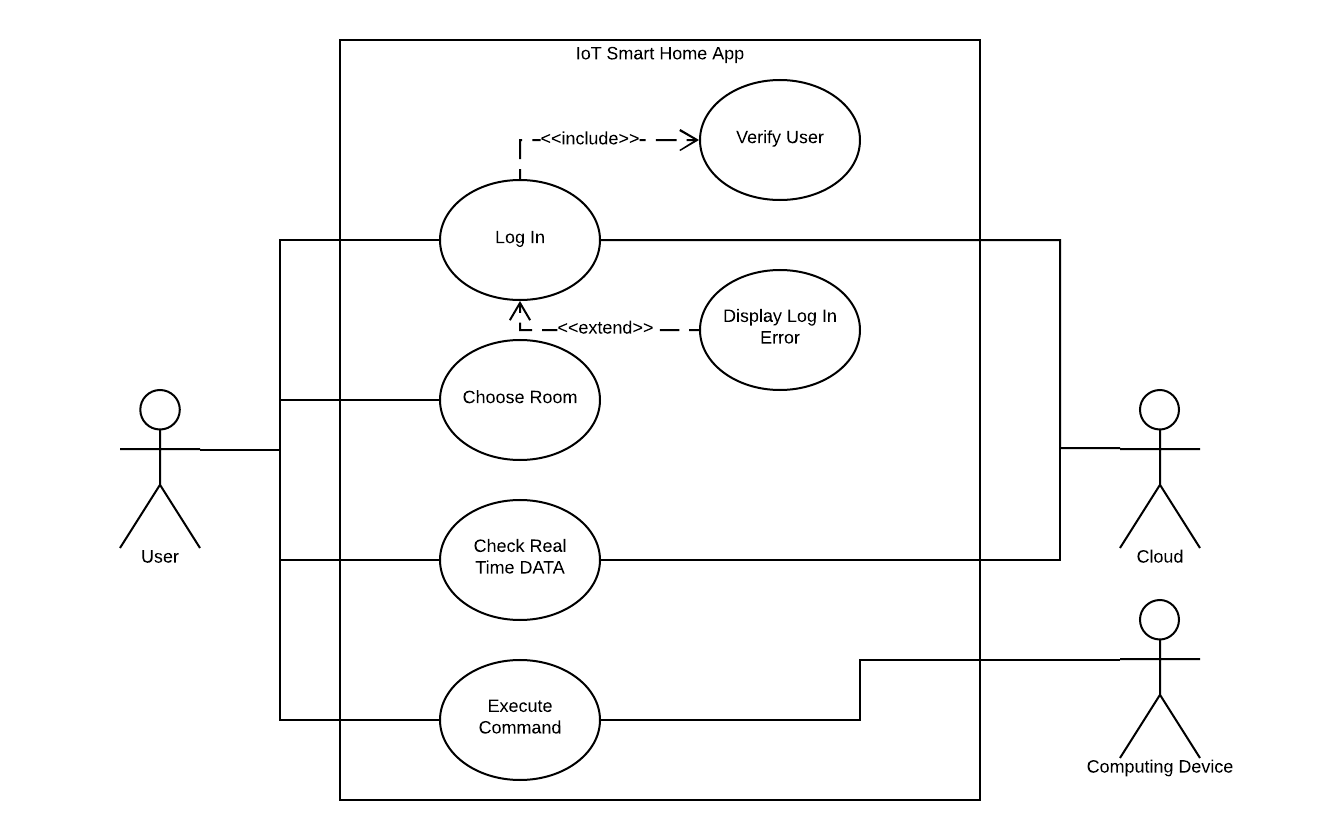
\includegraphics[width=1\textwidth]{use_case}
		\caption{Smart Home App Use Case Diagram.}
		\label{fig:ref_model}
	\end{center}
\end{figure}
       
\newpage
\subsection{IoT system architecture}

Lets start with the Figure 4, which represents Smart Home App Use Case Diagram. We can determine three main actors: 1) \textit{User}; 2) \textit{Cloud}; 3) \textit{Computing Device}. \textit{User} can Log In into the App, Choose Room to check DATA from and based on the data Execute Commands. \textit{Cloud} as an actor takes part in Log In and Checking Real Time DATA processes, while \textit{Computing Device} executes commands received from the \textit{User}.

\begin{figure} [H] %try to place the figure here (next option top of the page) 
	\begin{center}
		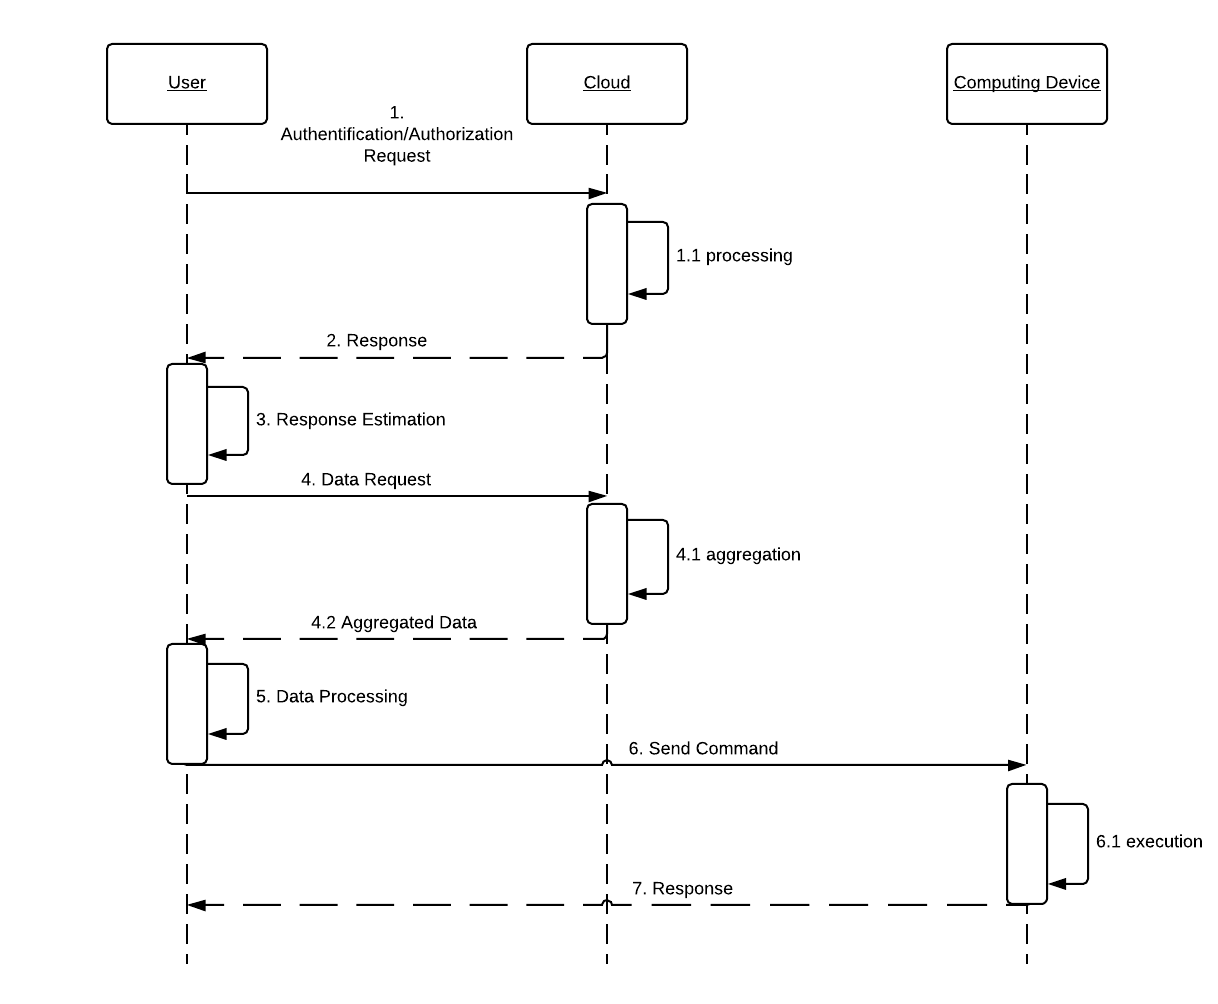
\includegraphics[width=1\textwidth]{App_SD}
		\caption{sHome App Sequence Diagram.}
		\label{fig:ref_model}
	\end{center}
\end{figure}

If we look at the Figure 5, we can see how the actors from the Figure 4 communicate with each other. \textit{User} sends authentication/authorization request with credentials to the \textit{Cloud}, which processes incoming request and, if credentials are matched, gives positive response to the \textit{User}, otherwise negative. Consequently, based on the \textit{Cloud's} response \textit{User} will be given an access to the Smart Home application functionality or asked to check Log In credentials. If the Log In processes finishes successful \textit{User} can request Real Time DATA from the \textit{Cloud}, which will be displayed in the App. After evaluating DATA \textit{User} can send command to the \textit{Computing Device}, which will then try to execute received command and provide \textit{User} with appropriate response message.     
 
\begin{figure} [H] %try to place the figure here (next option top of the page) 
	\begin{center}
		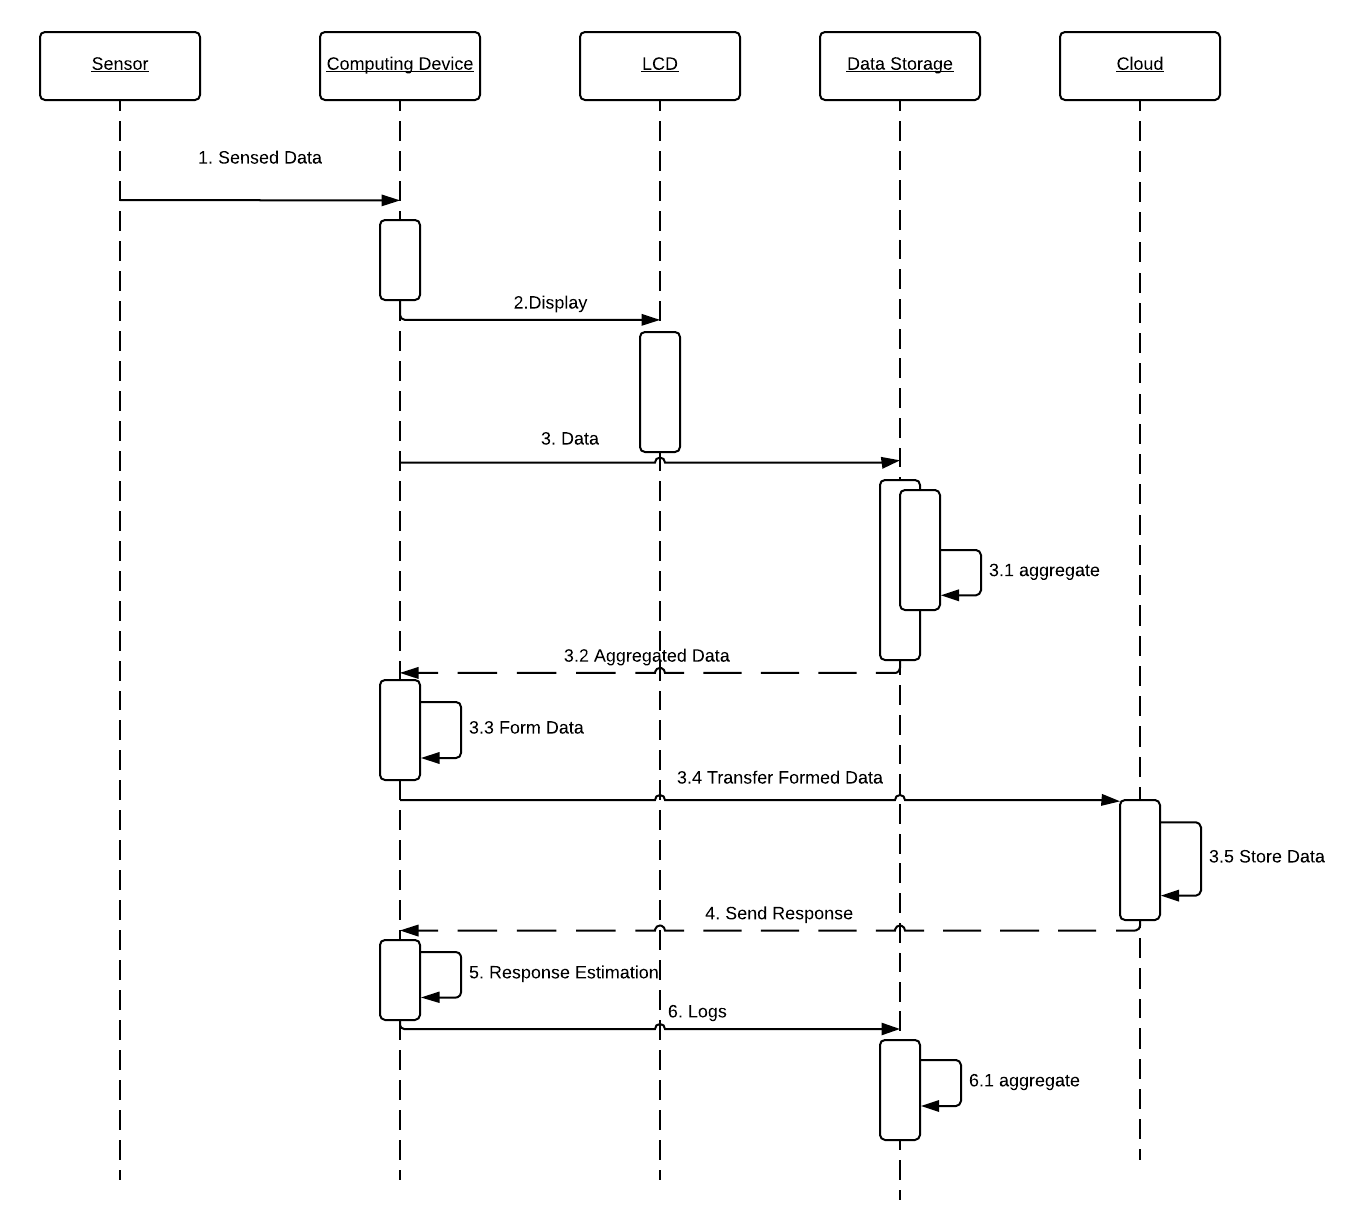
\includegraphics[width=1\textwidth]{IoT_SD}
		\caption{sHome IoT system Sequence Diagram.}
		\label{fig:ref_model}
	\end{center}
\end{figure}

Now lets dive dipper into the actual Smart Home IoT system architecture. From the Figure 6 we can see that actual work flow of the system starts from collecting Sensed Data from each available \textit{Sensor} in the system. Then this Data is displayed on \textit{LCD} screen, so you can monitor system state at home without using application. Sensed Data then is stored in local \text{Data Storage} and, when data from each sensor is aggregated, it is formed on \textit{Computing Device} and transfered to the \textit{Cloud}. On \textit{Cloud} data is stored in database and \textit{Computing Device} receives response from \textit{Cloud} if the data was stored successfully or not. Based on received response \textit{Computing Device} create Logs and store them in the local \textit{Data Storage} as a .log file.
     

     
	
\subsection{Application security}
\TODO{This subsection will explain how we will try to secure system and on which level. Will be based on previous subsections' info and personal contribution.}

\subsection{Testing results}
\TODO{This subsection will describe results of influencing system's work before and after applying previously developed security framework.}



\newpage
\section{Conclusion}


\newpage


% Use alternative local LaTeX bibliography

\begin{thebibliography}{9}
\tiny
\bibitem{FSSM} 
  Raimundas Matulevičius. 
  FundSecSysMod: Fundamentals of Secure System Modelling.
  \url{http://www.springer.com/gp/book/9783319617169#aboutBook}.
  (year 2017)
\bibitem{IoTRefMod}
	Martin Bauer, Nicola Bui, Jourik De Loof, Carsten Magerkurth, Andreas Nettsträter, Julinda Stefa, Joachim W. Walewski.
	IoTRefMod: Enabling Things to Talk ("IoT Reference Model" pp 113-162).
	\url{https://link.springer.com/book/10.1007/978-3-642-40403-0#about}.
  Publisher Name: Springer, Berlin, Heidelberg
  (year 2013)
\bibitem{MonSecIoT} 
	Anth 'ea Mayzaud, R 'emi Badonnel, and Isabelle Chrisment.
	MonSecIoT: Monitoring and Security for the Internet of Things.
	Universit 'e de Lorraine, LORIA, UMR 7503, France Inria Grand Est - Nancy, France.
	\url{https://link.springer.com/chapter/10.1007/978-3-642-38998-6_4}.
\bibitem{GSMA}
	GSMA Connected Living: Understanding the Internet of Things (IoT) (2014)
\bibitem{IoTSur}
	Fadele Ayotunde Alaba, Mazliza Othman, Ibrahim Abaker Targio Hashem, 	Faiz Alotaibi: Internet of Things security: A survey.
	Journal of Network and Computer Applications.
	Volume 88 Issue C, June 2017.
\bibitem{IoTSF} 
	Mahmoud Ammar, Giovanni Russello, Bruno Crispo: Internet of Things: A survey on the security of IoT frameworks.
	Journal of Information Security and Applications.
	Year 2017.
\bibitem{GUARD}
	The Guardian: DDoS attack that disrupted internet was largest of its kind in history, experts say. \url{https://www.theguardian.com/technology/2016/oct/26/ddos-
	attack-dyn-mirai-botnet}
	(2016)
\bibitem{SDN/NFV}
	Na Chen, Bo Rong, Abdel Mouaki, Wei Li: Self-Organizing Scheme Based on NFV and SDN Architecture for Future Heterogeneous Networks.
	Springer Science+Business Media New York 2015.
\bibitem{PRISMS}
	Abomhara, M., Koien: Security and Privacy in the Internet of Things: Current
	Status and Open Issues. In: International Conference on Privacy and Security in Mobile Systems (PRISMS), (2014)
\bibitem{IoTS}
	Alabaa, F.A., Othma, M., Abaker, I., Hashem, I.A.T., Alotaibib, F.: Internet of Things security: A survey. Journal of Network and Computer Applications 88(15), 10–28 (2017)
\bibitem{IoTCO}
	Mauro Conti, Ali Dehghantanha, Katrin Franke, Steve Watson: Internet of Things security and forensics: Chalenges and opportunities.
	Future Generation Computer Systems.
	Year 2017.
\bibitem{SSAIoT}
	Hui Li, Xin Zhou: Study on Security Architecture for Internet of Things.
	Haidian, Beijing, China.
	ICAIC 2011: Applied Informatics and Communication pp 404-411. 
\bibitem{ICAIC}
	Li, H., X., Z.: Study on Security Architecture for Internet of Things. In: ICAIC 2011, Part I. vol. CCIS 224, pp. 404–411 (2011)
\bibitem{EMS}
	Hellaoui, H., Koudil, M., Bouabdallah, A.: Energy-efficient mechanisms in security of the internet of things: A survey. Computer Networks 127, 173–189 (2017)
\bibitem{Concept}
	Irene Mavrommati, George Birbilis, John Darzentas: A conceptual framework for the design of IoT architectures that support end-user development.
	Networking Science: December 2013, Volume 3, Issue 1–4, pp 71–81.
\bibitem{SEA}
	Sanaz Rahimi Moosavi, Tuan Nguyen Gia, Amir-Mohammad Rahmani, Ethiopia Nigussie, Seppo Virtanen, Jouni Isoaho, Hannu Tenhunen: SEA: A Secure and Efficient Authentication and Authorization Architecture for IoT-Based Healthcare Using Smart Gateways.
	6th International Conference on Ambient Systems, Networks and Technologies.
	Year 2015.
	\url{https://www.sciencedirect.com/science/article/pii/S1877050915008133#!}
\bibitem{DCN}
	Banerjee, M., Lee, J., R., C.K.K.: A blockchain future to Internet of Things security: A position paper. Digital Communications and Networks (2018)
\bibitem{SAD}
	Dubois, E., Heymans, P., Mayer, N., Matuleviˇcius, R.: A Systematic Approach to Define the Domain of Information System Security Risk Management, pp. 289–306. Springer (2010)
\bibitem{Cloud}
	Nick Antonopoulos, Lee Gillam: Cloud Computing: Principles, Systems and Applications.
	Springer-Verlag London Limited 2010.
\bibitem{IoTSecChel}
	Qi Jing, Athanasios V. Vasilakos, Jiafu Wan, Jingwei Lu, Dechao Qiu: Security of the Internet of Things: perspectives and challenges
	17 June 2014.
	Springer Science+Business Media New York 2014.
	\url{https://link.springer.com/content/pdf/10.1007%2Fs11276-014-0761-7.pdf}
\bibitem{MSM}
	Yang, X., Li, Z., Geng, Z., Zhang, H.: A Multi-layer Security Model for Internet of Things. In: IOT Workshop 2012. vol. CCIS 312, pp. 388–393 (2012)
\bibitem{IoTF}
	Ammar, M., Russello, G., B., C.: Internet of Things: A survey on the security of IoT frameworks. Journal of Information Security and Applications 38, 8–27 (2018)
\bibitem{SE}
	Thomas Kirste: Smart Environments: True Visions.
	Springer-Verlag Berlin Heidelberg 2006.
\bibitem{ITS}
	Joseph M. Sussman: Perspectives on Intelligent Transportation Systems (ITS).
	Massachusetts Institute of Technology
	Cambridge, Massachusetts.
	Year 2005.
\bibitem{IoTICA}
	Vipindev Adat, B. B. Gupta: Security in Internet of Things: issues, challenges, taxonomy, and architecture.
	13 June 2017.
	© Springer Science+Business Media, LLC 2017.
	\url{https://link.springer.com/content/pdf/10.1007%2Fs11235-017-0345-9.pdf}
\bibitem{SOA}
	Valérie Issarny, Georgios Bouloukakis, Nikolaos Georgantas, Benjamin Billet: Revisiting Service-Oriented Architecture for the IoT: A Middleware Perspective.
	ICSOC 2016: Service-Oriented Computing pp 3-17
	20 September 2016.
\bibitem{SH}
	Zahrah A. Almusaylim, Noor Zaman: A review on smart home present state and challenges: linked to context-awareness internet of things (IoT)
	\url{https://link.springer.com/article/10.1007/s11276-018-1712-5}
\bibitem{SecIoT} 
	Rodrigo Roman, Pablo Najera, and Javier Lopez.
	SecIoT: Securing the Internet of Things.
	University of Malaga, Spain.
	\url{https://www.nics.uma.es/pub/papers/1633.pdf}
\bibitem{SmartC}
	Viviana Bastidas, Marija Bezbradica, Markus Helfert: Cities as Enterprises: A Comparison of Smart City Frameworks Based on Enterprise Architecture Requirements. 
	26 May 2017.
\bibitem{RheoStat}
	Ashish Gehani and Gershon Kedem.
	RheoStat: Real-Time Risk Management.
	Department of Computer Science, Duke University.
	\url{https://link.springer.com/chapter/10.1007/978-3-540-30143-1_16}
\bibitem{SMG}
	Kwang-Ryul Jung, Aesoon Park, and Sungwon Lee: Machine-Type-Communication (MTC) Device Grouping: Algorithm for Congestion Avoidance of MTC Oriented
	LTE Network.
	 Springer-Verlag Berlin Heidelberg 2010.
\bibitem{UnderIoT}
	GSM Assosiation.
	UnderIoT: Understanding the Internet of Things (IoT).
	July 2014.
	\url{https://www.gsma.com/iot/wp-content/uploads/2014/08/cl_iot_wp_07_14.pdf}
\bibitem{GDMA}
	Rebika Rai, Chunkey Lepcha, Partha Pratim Ray, Prashant Chettri.
	GDMA: General Domain Model Architecture of the IoT.
	October 2013.
	\url{https://www.researchgate.net/publication/259497112_GDMA_Generalized_Domain_Model_Architecture_of_Internet_of_Things}
\bibitem{CORAS}
	Theo Dimitrakos, Juan Bicarregui and Ketil Stølen.
	CORAS: CORAS - A Framework for Risk Analysis of Security Critical Systems.
	April 2002.
	\url{https://www.ercim.eu/publication/Ercim_News/enw49/dimitrakos.html}
\bibitem{EBIOS}
	EBIOS: EBIOS -  is a method for analysis, evaluation and action on risks relating to information systems.
	Year 2000.
	\url{https://en.wikipedia.org/wiki/EBIOS}
\bibitem{AURUM}
	Andreas Ekelhart, Stefan Fenz and Thomas Neubauer.
	AURUM: AURUM - A Framework for Information Security Risk Management
	Year 2009.
	\url{https://pdfs.semanticscholar.org/f107/871d55daba22e55d0afe594c19339d882cb9.pdf}
\bibitem{MEHARI}
	MEHARI: MEHARI - MEthod for Harmonized Analysis of RIsk.
	Year 2010.
	\url{https://en.wikipedia.org/wiki/MEHARI}
\bibitem{CRAMM}
	SANS Institute.
	CRAMM: CRAMM - A Qualitative Risk Analysis and Management Tool.
	\url{https://www.sans.org/reading-room/whitepapers/auditing/qualitative-risk-analysis-management-tool-cramm-83}
\bibitem{OWASP}
	OWASP: OWASP - Open Web Application Security Project  is a 501(c)(3) worldwide not-for-profit charitable organization focused on improving the security of software.
	\url{https://www.owasp.org/index.php/Main_Page}
\bibitem{XSS}
	XSS: XSS - Cross-site Scripting.
	\url{https://www.owasp.org/index.php/Cross-site_Scripting_(XSS)} 
\bibitem{SQLi}
	SQLi: SQLi - SQL injection is a code injection technique, used to attack data-driven applications.
	\url{https://en.wikipedia.org/wiki/SQL_injection}
\bibitem{CSRF}
	CSRF: CSRF - Cross-site request forgery, also known as one-click attack or session riding.
	\url{https://en.wikipedia.org/wiki/Cross-site_request_forgery}
\bibitem{BufOver}
	BufOver: BufOver -  Buffer overflow, or buffer overrun, is an anomaly where a program, while writing data to a buffer, overruns the buffer's boundary and overwrites adjacent memory locations.
	\url{https://en.wikipedia.org/wiki/Buffer_overflow}
\bibitem{FuzA}
	FuzA: FuzA -  Fuzz testing or Fuzzing is a Black Box software testing technique.
	\url{https://www.owasp.org/index.php/Fuzzing}
\bibitem{DoS}
	DoS: DoS - Denial-of-service attack.
	\url{https://en.wikipedia.org/wiki/Denial-of-service_attack}
\bibitem{SSL/TLS}
	SSL/TLS: SSL/TLS - Secure Sockets Layer/Transport Layer Security.
	\url{https://en.wikipedia.org/wiki/Transport_Layer_Security}
\bibitem{MQTT}
	MQTT: MQTT - Message Queue Telemetry Transport.
	\url{https://www.hivemq.com/blog/mqtt-security-fundamentals-payload-encryption}
\bibitem{CO}
	CO: CO - Code obfuscation.
	\url{https://www.ncsc.gov.uk/content/files/protected_files/guidance_files/Code-obfuscation.pdf}
\bibitem{SB}
	SB: SB - Secure Boot.
	\url{https://docs-old.fedoraproject.org/en-US/Fedora/18/html/UEFI_Secure_Boot_Guide/chap-UEFI_Secure_Boot_Guide-What_is_Secure_Boot.html}
\bibitem{INT}
	The Internet: This article about the worldwide computer network. 
	 Wikipedia, the free encyclopedia.
	\url{https://en.wikipedia.org/wiki/Internet}
\bibitem{V}
	V: V - Vulnerability in terms of cyber-security.
	\url{https://www.techopedia.com/definition/13484/vulnerability} 
\bibitem{Ex1}
	 Ex1: Ex1 - Mirai botnet.
	 \url{https://www.theguardian.com/technology/2016/oct/26/ddos-attack-dyn-mirai-botnet}
\bibitem{Ex2}
	Mathews, L.: Hackers Use DDoS Attack To Cut Heat To Apartments.
	\url{https://www.forbes.com/sites/leemathews/2016/11/07/ddos-attack-leaves-finnish-apartments-without-heat/#45631d451a09}
\bibitem{Ex3}
	Weagle, S.: IoT-Driven Botnet Attacks US University.
	\url{https://www.corero.com/blog/798-iot-driven-botnet-attacks-us-university.html}
\bibitem{Ex4}
	Khandelwal, S.: Two Romanians Charged with Hacking Police CCTV Cameras Before Trump Inauguration.
	\url{https://thehackernews.com/2017/12/police-camera-hacking.html}
\bibitem{Ex5}
	Greenberg, A.: Hackers Remotely Kill a Jeep on the Highway - with me in it.
	\url{https://www.wired.com/2015/07/hackers-remotely-kill-jeep-highway/}
\bibitem{Ex6}
	Carolina: Goodbye Spy Toy: Germany Bans My Friend Cayla Doll.
	\url{https://www.hackread.com/good-bye-spying-toy-germany-bans-my-friend-cayla-doll/}
\end{thebibliography}


\newpage
%\appendix
%\section*{\appendixname}
\iflanguage{english}%
  {\section*{Appendix}
  \addcontentsline{toc}{section}{Appendix}
  }


\section*{I. Glossary}
\addcontentsline{toc}{subsection}{I. Glossary}

\newpage


\section*{II. Licence}

\addcontentsline{toc}{subsection}{II. Licence}

\subsection*{Non-exclusive licence to reproduce thesis and make thesis public}

I, \textbf{Shapaval Raman},

\begin{enumerate}
\item
herewith grant the University of Tartu a free permit (non-exclusive licence) to:
\begin{enumerate}
\item[1.1]
reproduce, for the purpose of preservation and making available to the public, including for addition to the DSpace digital archives until expiry of the term of validity of the copyright, and
\item[1.2]
make available to the public via the web environment of the University of Tartu, including via the DSpace digital archives until expiry of the term of validity of the copyright,
\end{enumerate}

of my thesis

\textbf{Security Risk Management for the IoT systems}

supervised by Raimundas Matulevicius

\item
I am aware of the fact that the author retains these rights.
\item
I certify that granting the non-exclusive licence does not infringe the intellectual property rights or rights arising from the Personal Data Protection Act. 
\end{enumerate}

\noindent
Tartu, dd.mm.yyyy





\end{document}

